% https://www.springer.com/gp/computer-science/lncs/conference-proceedings-guidelines
% LLNCS macro package for Springer Computer Science proceedings;
% Version 2.20 of 2017/10/04
\documentclass[runningheads]{llncs}

\usepackage{graphicx}
\usepackage{multirow}
\usepackage{bbding}
\usepackage{color}
\usepackage{authblk}
\usepackage{blindtext}
\usepackage{url}
\usepackage{fancyhdr}

%%%%%%%%%%%%%%%%%%%%%%%%%%%%%%%%%%%%%%%%%%%%%%%%
% ページスタイル
%%%%%%%%%%%%%%%%%%%%%%%%%%%%%%%%%%%%%%%%%%%%%%%%
\pagestyle{fancy}
    \renewcommand{\headrulewidth}{0pt}
    \renewcommand{\footrulewidth}{1pt}
    \lhead{}
    \chead{}
    \rhead{}
    \lfoot{\footnotesize\textit{Persuasive 2022, Adjunct Proceedings of the 17th International Conference on Persuasive Technology. Copyright © 2022 for this paper by its authors. Use permitted under Creative Commons License Attribution 4.0 International (CC BY 4.0).}}
    \cfoot{}
    \rfoot{}

\fancypagestyle{kisuu}{\lhead{}
    \chead{}
    \rhead{\thepage}
    \fancyfoot{}
    \renewcommand{\footrulewidth}{0pt}}

\fancypagestyle{guusuu}{\lhead{\thepage\qquad\quad Y. Ohira et al.}
    \chead{}
    \rhead{}
    \fancyfoot{}
    \renewcommand{\footrulewidth}{0pt}}


\begin{document}

\title{
  Design and development of appendable elevator monitoring system to nudge people behavior change
}

\author{
  Yuta Ohira\inst{1}\orcidID{0000-0002-9251-242X} \and
  Yugo Nakamura\inst{1}\orcidID{0000-0002-8834-5323} \and
  Yutaka Arakawa\inst{1}\orcidID{0000-0002-7156-9160}
}

\authorrunning{Y. Ohira et al.}
\titlerunning{Appendable elevator monitoring system to nudge people behavior change}

\institute{
  Kyushu University, Fukuoka, Japan
}

\maketitle

% show footnote
\thispagestyle{fancy}

%%%%%%%%%%%%%%%%%%%%%%%%%%%%%%%%%%%%%%%%%%%%%%%%
% 概要
%%%%%%%%%%%%%%%%%%%%%%%%%%%%%%%%%%%%%%%%%%%%%%%%

\begin{abstract}
  % Due to the impact of the COVID-19, there has been a growing interest in visualizing the degree of congestion in public transportation and restaurants. Trains, buses, restaurants, and elevators are some of the places that tend to be crowded.

  % In this study, we developed a system to visualize the number of people in the elevator and the degree of congestion on each floor to the users to reduce the congestion in the elevator. The main purpose of this system is to present the congestion status in the elevator to the people who are waiting for the elevator, and to nudge them to make a decision such as to use the stairs or to delay the timing of pushing the elevator up/down button.

  % In some high-rise condominiums and large commercial facilities, cameras are installed in the elevators, and the images captured by the cameras are displayed on signage in the elevator halls. However, the camera-based method has some problems such as invasion of privacy and installation cost of the signage, and there are some places where large-scale construction cannot be done due to the structure of the building. Therefore, we propose a system that uses Bluetooth Low Energy (BLE) signals instead of cameras to measure the degree of congestion to ensure privacy, and that can be easily appended to most elevators.

  In this study, we propose a behavior change support system that encourages people to use stairs instead of elevators. Using the stairs is not only good for one's health, but nowadays it also plays a role in dense avoidance from the perspective of COVID-19.

  Although many people are waiting for the elevator, we thought that if we knew how many people were on the elevator, more people could change their behavior. However, there are few buildings where the number of people in the elevator is displayed on each floor. So, we have developed a headcount measurement system in the cargo and a visualization system, those can be easily appended to the current elevator.

  As a method to measure the number of people in an elevator, we propose a method to detect BLE signals transmitted from the terminals of elevator users who have installed COCOA, an application for confirming contact with the COVID-19 in Japan, and to measure in real time the number of detected BLE signals with a received signal strength (RSSI) exceeding a certain value. We propose a method to measure the number of BLE signals detected in real time.

  In this paper, we have designed and developed the system, verified the accuracy of the detection of the continuous operation time and the number of passengers, and estimated the behavior pattern and waiting time of elevator users using the system. The evaluation of the transformation of the decision making of the elevator users brought about by this system is out of the scope of this paper and will be discussed in the future.

  \keywords{Elevator \and Signage \and Nudge \and BLE \and COCOA}
\end{abstract}

%%%%%%%%%%%%%%%%%%%%%%%%%%%%%%%%%%%%%%%%%%%%%%%%%%%%%%%%%%%%%%%%%%%%%%%%
% 1. はじめに
%%%%%%%%%%%%%%%%%%%%%%%%%%%%%%%%%%%%%%%%%%%%%%%%%%%%%%%%%%%%%%%%%%%%%%%%
\section{Introduction}
Due to the impact of the COVID-19, it is becoming more important to avoid the crowded places. Trains, buses, restaurants, and elevators tend to be crowded with people. Efforts are being actively made to visualize the congestion in these places and to prevent people from being led to the congested places. In this paper, we focus on the visualization of the congestion level of elevators. The fact that elevators are places where people tend to be crowded is mentioned in a poster by the Ministry of Health, Labor and Welfare of Japan to prevent the spread of the COVID-19\cite{ministry}. The elevator is very narrow and easily crowded. Also, it is difficult for elevator users to avoid congestion. Even if the elevator is not crowded at the time when the user gets on, if many people get on at the intermediate floor, the user who was originally on the elevator will not get off unless the floor is the destination floor. In the opposite pattern, if a user presses the elevator button and waits for the elevator, but the elevator is crowded, the user may give up and wait for the next elevator or be forced to get on. This is considered to be an incident that occurs because the user cannot grasp the status of each floor and the number of people in the elevator at the timing when the elevator button is pressed. If there are users on each floor as described above, the elevator will stop at each floor, which will lead to deterioration of the transportation efficiency of the elevator and increase of the waiting time.


% 図:システム概要
% TODO: 図中の説明は、英語のものに変更する
\begin{figure}[t]
\begin{center}
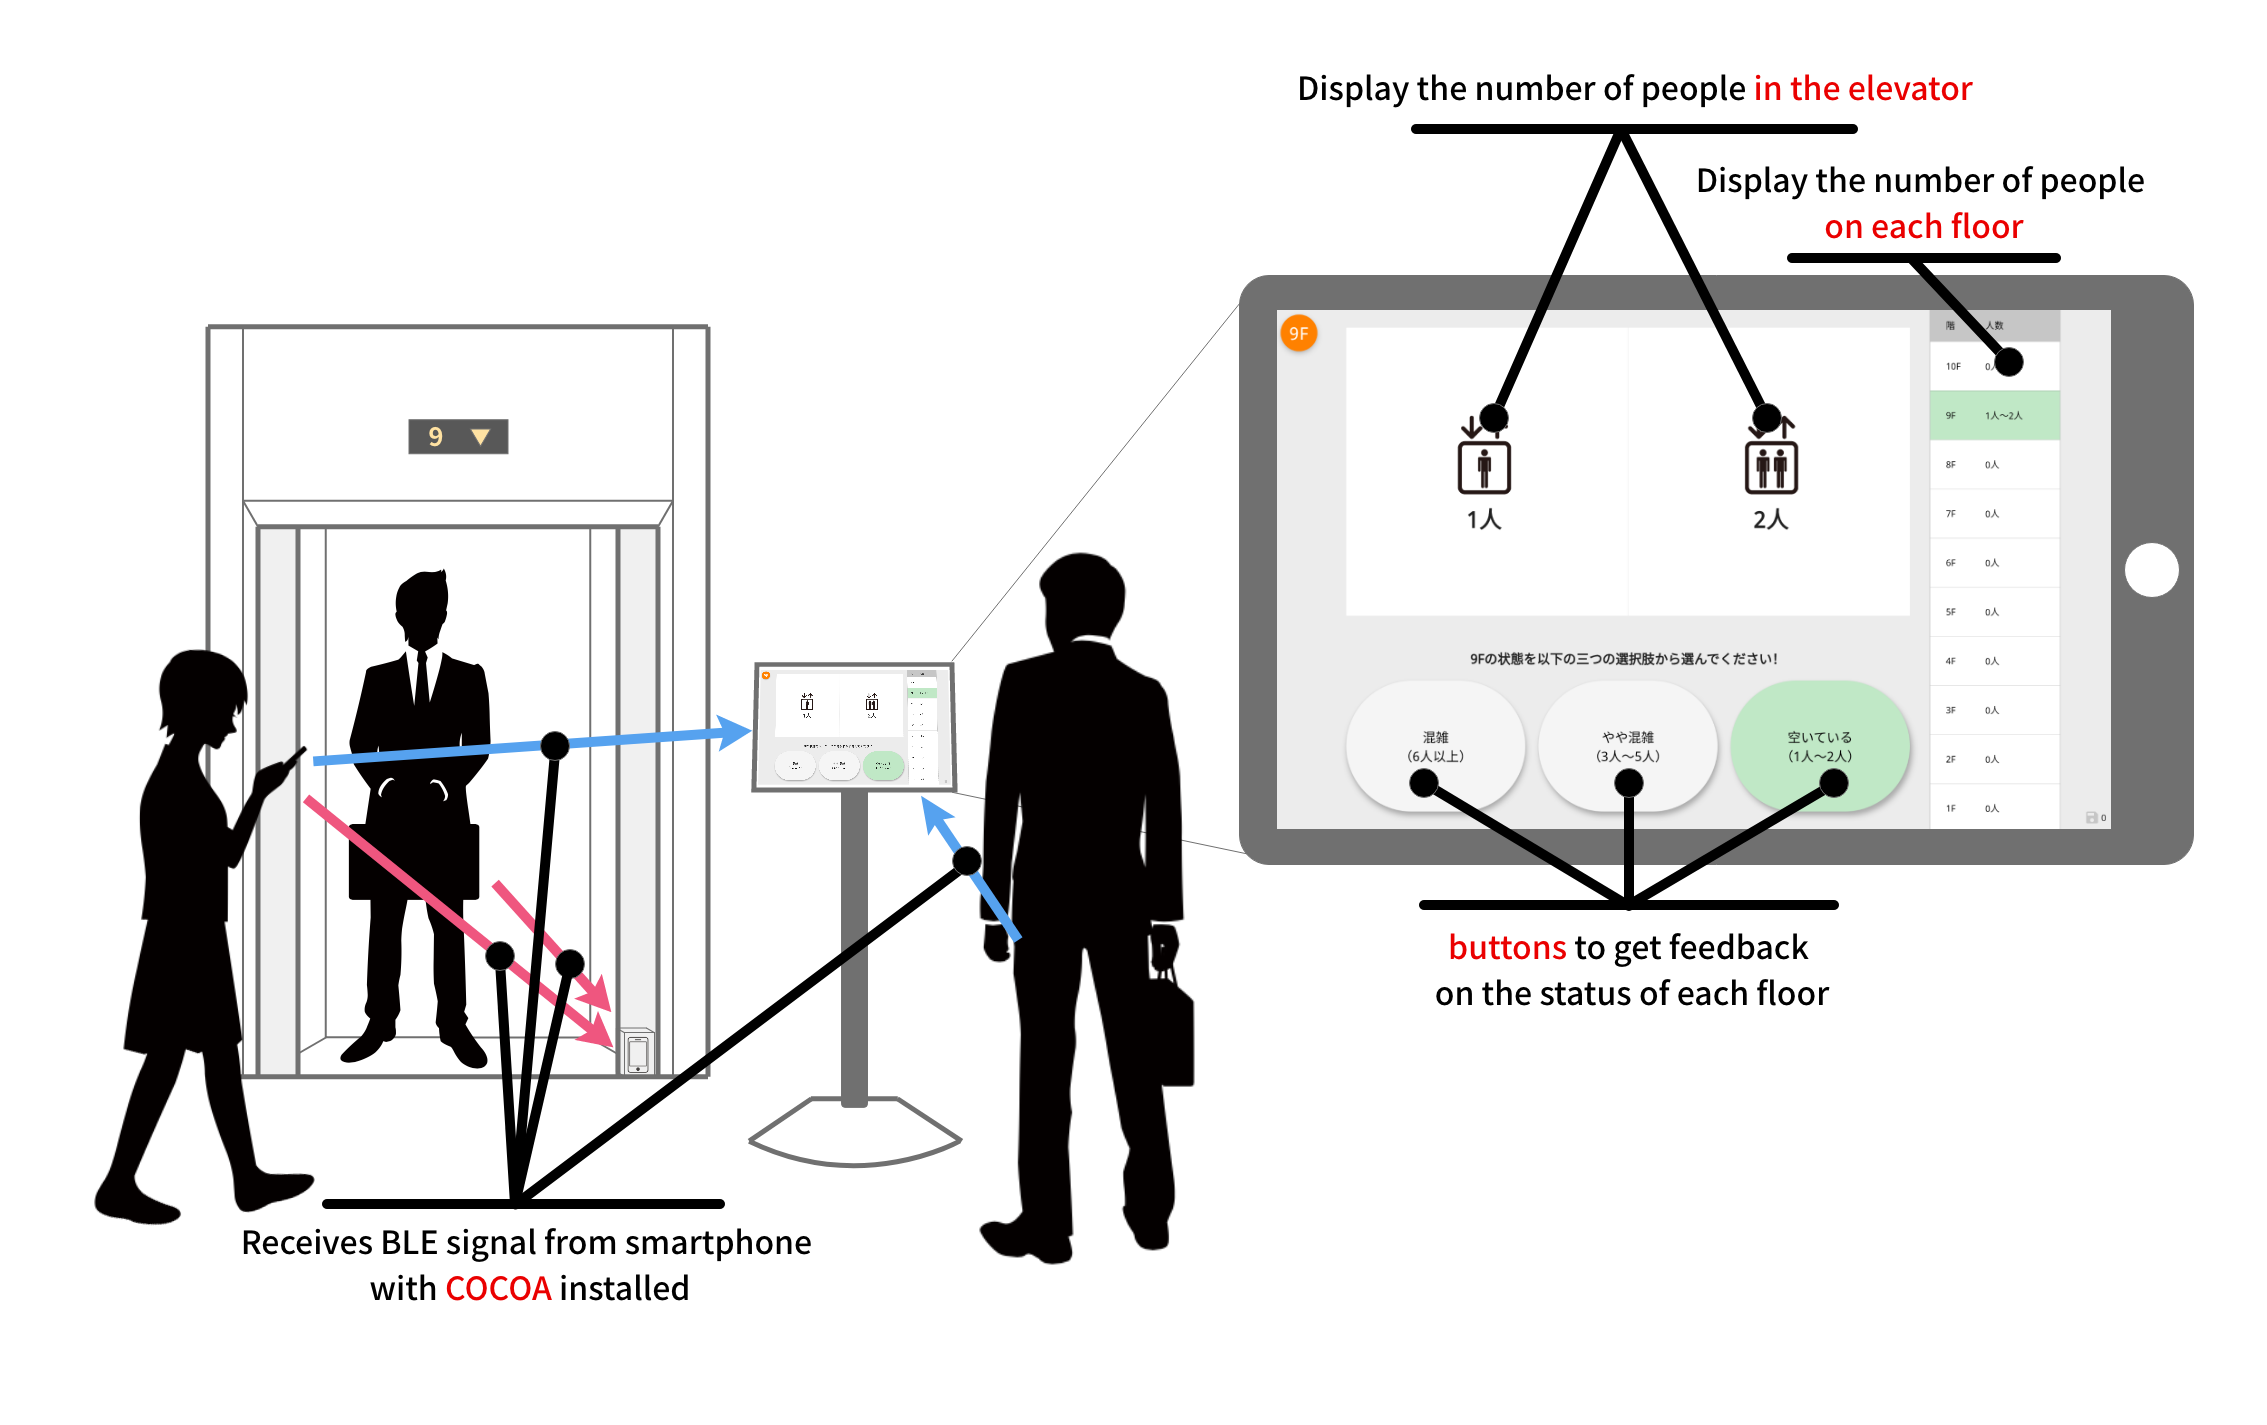
\includegraphics[clip, width=1.0\hsize]{img/system.png}
\caption{System Overview}
\label{fig:system}
\end{center}
\end{figure}


To solve these problems, a method of informing users of the congestion status of elevators through a smartphone application has been proposed by building company, kajima\cite{kajima}. The method using a smartphone application requires the user to install an application, which raises the hurdle to grasp the congestion information. In addition, kajima\cite{kajima} proposes a method for detecting passengers by using a camera as a method to grasp the congestion status in an elevator.
Although the camera-based detection is highly accurate, there are some problems in terms of installation cost, such as privacy issues and the need to install a ceiling. In another approach, a gate is installed in front of the elevator and an ID card is scanned to allow the system to know the number of elevator users and their destinations, and to select the optimal elevator and timing for boarding\cite{elenavi}. Since the number of elevator users is controlled by the gate, it is easy to control the number of elevator users and to eliminate the congestion in the elevators. 

In this study, we propose a appendable system in which a tablet terminal is installed in front of the elevator to present the number of people in the elevator, the congestion status of each floor (Figure \ref{fig:system}). We believe that this system will solve the problem of not being able to grasp the status of other floors and the number of people in the elevator at the time when the elevator button is pressed, which is a problem unique to elevators. Compared with the method of having users install an application, this system allows users to easily obtain information on congestion, and thus encourages them to make decisions such as using the stairs or waiting for the next elevator before pressing the elevator button. 

As a part of the basic experiment, we also evaluated the continuous operation time and detection accuracy of the system, and estimated the behavior pattern and waiting time of the elevator users based on the RSSI time series data of BLE signals acquired from the system.

This paper is organized as follows. In Chapter 2, related research is described, and in Chapter 3, the outline and requirements of the elevator usage visualization system are described. In Chapter 4, the estimation of the user's behavior pattern and waiting time using the system is explained. Finally, in Chapter 5, we conclude this paper and discuss future issues.

%%%%%%%%%%%%%%%%%%%%%%%%%%%%%%%%%%%%%%%%%%%%%%%%%%%%%%%%%%%%%%%%%%%%%%%%
% 2. 関連研究
%%%%%%%%%%%%%%%%%%%%%%%%%%%%%%%%%%%%%%%%%%%%%%%%%%%%%%%%%%%%%%%%%%%%%%%%
\section{Related Research}

In designing a congestion visualization system, the process of determining the method for measuring and estimating the congestion level and the method for communicating and visualizing the congestion information to users is important. In this chapter, we will first discuss the research on congestion measurement and general services and researches on congestion visualization, and then we will discuss the status of this research, mentioning the efforts and current status of sensing using IoT(Internet of Things) in elevators. The comparison between the related work and our proposed system is summarized in Table \ref{table:related_work}.


% 表:関連研究
\begin{table*}[bt]
\centering
\caption{Summary of related research on crowded estimation and crowded visualization and our proposed system}
\begin{tabular}{ccccc} \hline
\textbf{Year} & 
\textbf{Reference} &
\textbf{Sensor} & % センサー
\textbf{Target} & % 対象
\textbf{User Burden} % ユーザーの負担
\\
\hline \hline
2009 & \cite{research_elevator_camera} & Camera & Elevator users & - \\
2014 & \cite{research_camera} & Camera & People and Crowds & - \\
2016 & \cite{komai2016beacon} & BLE & \begin{tabular}{c}People in \\ elderly facilities\end{tabular} & Have a BLE beacon \\
2016 & \cite{komai2016elderly} & BLE & \begin{tabular}{c}People in \\ elderly facilities\end{tabular} & Have a BLE beacon \\
2018 & \cite{umeki2018real} & BLE & Sightseer & Have a BLE beacon \\
2019 & \cite{misc/26987957} & BLE \& WiFi & Sightseer & Install Application \\
2020 & \cite{research_itocon} & BLE \& WiFi & People and Crowds & - \\
2020 & \cite{ipsj-taikai-2020-matsumoto} & WiFi & People in the room & - \\
2021 & \cite{kanamitu-2021-dicomo} & BLE & Bus users & Install COCOA \\
2021 & \cite{kajima} & Camera \& BLE & Elevator users & Install Application \\
2021 & \cite{elenavi} & - & Elevator users & - \\
2021 & \begin{tabular}{c}our proposed \\ system\end{tabular} & BLE & Elevator users & Install COCOA \\
\hline
\end{tabular}
\label{table:related_work}
\end{table*}


% 混雑度計測に関する研究
\subsection{Research on congestion measurement}

A method to detect crowds by image processing using a camera has been proposed\cite{research_camera}. When using a camera, privacy must be taken into account. In addition, since power supply is often unavailable in elevators, it is difficult to operate the camera method on battery power all day long due to power consumption issues.
As a low power consumption method for measuring congestion, we have developed a method using WiFi CSI (Channel State Information) \cite{ipsj-taikai-2020-matsumoto} and a method for estimating congestion based on the RSSI distribution of BLE signals \cite{misc/26987957}\cite{umeki2018real}. However, all of them measure the degree of congestion in the target environment from the attenuation of radio waves by installing transmitters and receivers across the measurement environment, which requires a large indoor or outdoor space or installing devices in opposite directions. 

In this study, we apply a method that utilizes signals transmitted by COCOA, the Contact-Confirming Application in Japan, which is based on ''exposure notification system'' codeveloped by Google and Apple. Exposure Notification is a decentralized reporting based protocol built on a combination of Bluetooth Low Energy technology and privacy-preserving cryptography. In recent smartphone operating systems, background operation is severely restricted, so it is no longer possible to create applications that continuously transmit BLE signals. Even if it were possible, it would be difficult to have a large number of people install it. COCOA, on the other hand, has already been installed by a certain number of people, and continuous background operation is specially permitted for iOS and Android.

Examples of the use of COCOA to measure congestion include the campus congestion visualization system itocon, which has been in operation in our laboratory since June 2020, \cite{research_itocon}, and an example of its use for sensing congestion in a bus \cite{kanamitu-2021-dicomo}. In this method, only one device needs to be installed in the environment, and no application needs to be installed on the user side. The disadvantage is that not all users have COCOA installed.


% 混雑度可視化に関するサービスや研究
\subsection{Services and research on congestion visualization}

Congestion visualization can be summarized in terms of macro and micro. From the macroscopic perspective, Google Maps and Yahoo! Map applications have started around 2015. These services were discontinued in January 2020, but have been revived again due to the Corona disaster. These services are measured based on the information of the users of Google and Yahoo! In order to visualize the degree of restraint in going out during the Corona disaster, congestion visualization services provided by cell phone companies, such as Docomo's Mobile Spatial Statistics and Softbank's Agoop, are also gaining recognition. These services visualize the rough congestion level on a 500m mesh scale.

From a microscopic point of view, the Corona disaster has made it possible to display train congestion levels in transfer guides \footnote{The ''Congestion Forecast'' function, which allows you to quickly understand the trend of train congestion, is now available~\url{https://blog-transit.yahoo.co.jp/info/20200601.html}}. As for the level of congestion per store, a company called VACAN\footnote{VACAN~\url{https://corp.vacan.com/}} has emerged. 

However, since only the users in the building need the information about the elevators, it seems that no one other than the elevator companies measure or visualize the congestion level.


% エレベータにおけるIoTを用いたセンシングの取り組みと現状
\subsection{Approaches of IoT-Based Sensing in Elevators}

Some of the latest elevators are already equipped with signage that measures the number of people using cameras and weight scales, and displays the number of people in the elevator and the images from the cameras to people waiting for the elevator. However, most ordinary elevators are not equipped with such signage. Also, elevators cannot be replaced easily, so it is difficult to install them except in the latest buildings or commercial facilities. Furthermore, even in the latest buildings, such high-end elevators are not always installed due to cost and demand issues. In fact, Ito Campus of Kyushu University started construction in 2005, but at present (November 2021), we cannot find any high-end elevator with signage installed in the campus. In the case of apartments, cameras are installed in the elevators for the purpose of monitoring suspicious persons, and there are displays in the elevator halls that show the images from the cameras. While we may spend a lot of money for security, we do not often spend a lot of money to install signage to relieve congestion.


% 本研究の位置付け
\subsection{The position of this research}

This research aims to realize a status sensing and visualization system that can be retrofitted and easily installed in existing popular elevator systems. Although not included in this paper, we aim to support decision making, such as choosing to use the stairs instead of waiting for the train to board, and is not intended to be applied to high-rise buildings, but to buildings with a height that can be reached by stairs.

%%%%%%%%%%%%%%%%%%%%%%%%%%%%%%%%%%%%%%%%%%%%%%%%%%%%%%%%%%%%%%%%%%%%%%%%
% 3. エレベータ利用状況可視化システム
%%%%%%%%%%%%%%%%%%%%%%%%%%%%%%%%%%%%%%%%%%%%%%%%%%%%%%%%%%%%%%%%%%%%%%%%
\section{A System for Visualizing Elevator Usage}

In this chapter, we explain the system diagram Figure \ref{fig:system} for visualizing the number of people in the elevator and the number of people on each floor. 

% システム要件
\subsection{System Requirement}

To realize this system, the following requirements are necessary.

\begin{quote}
 \begin{itemize}
  \item Requirement 1: Obtain the number of people in the elevator and the status of the elevator hall on each floor.
  \item Requirement 2: Visualization of the information obtained in Requirement 1 for elevator users
 \end{itemize}
\end{quote}

% 図:システム2
\begin{figure}[t]
\begin{center}
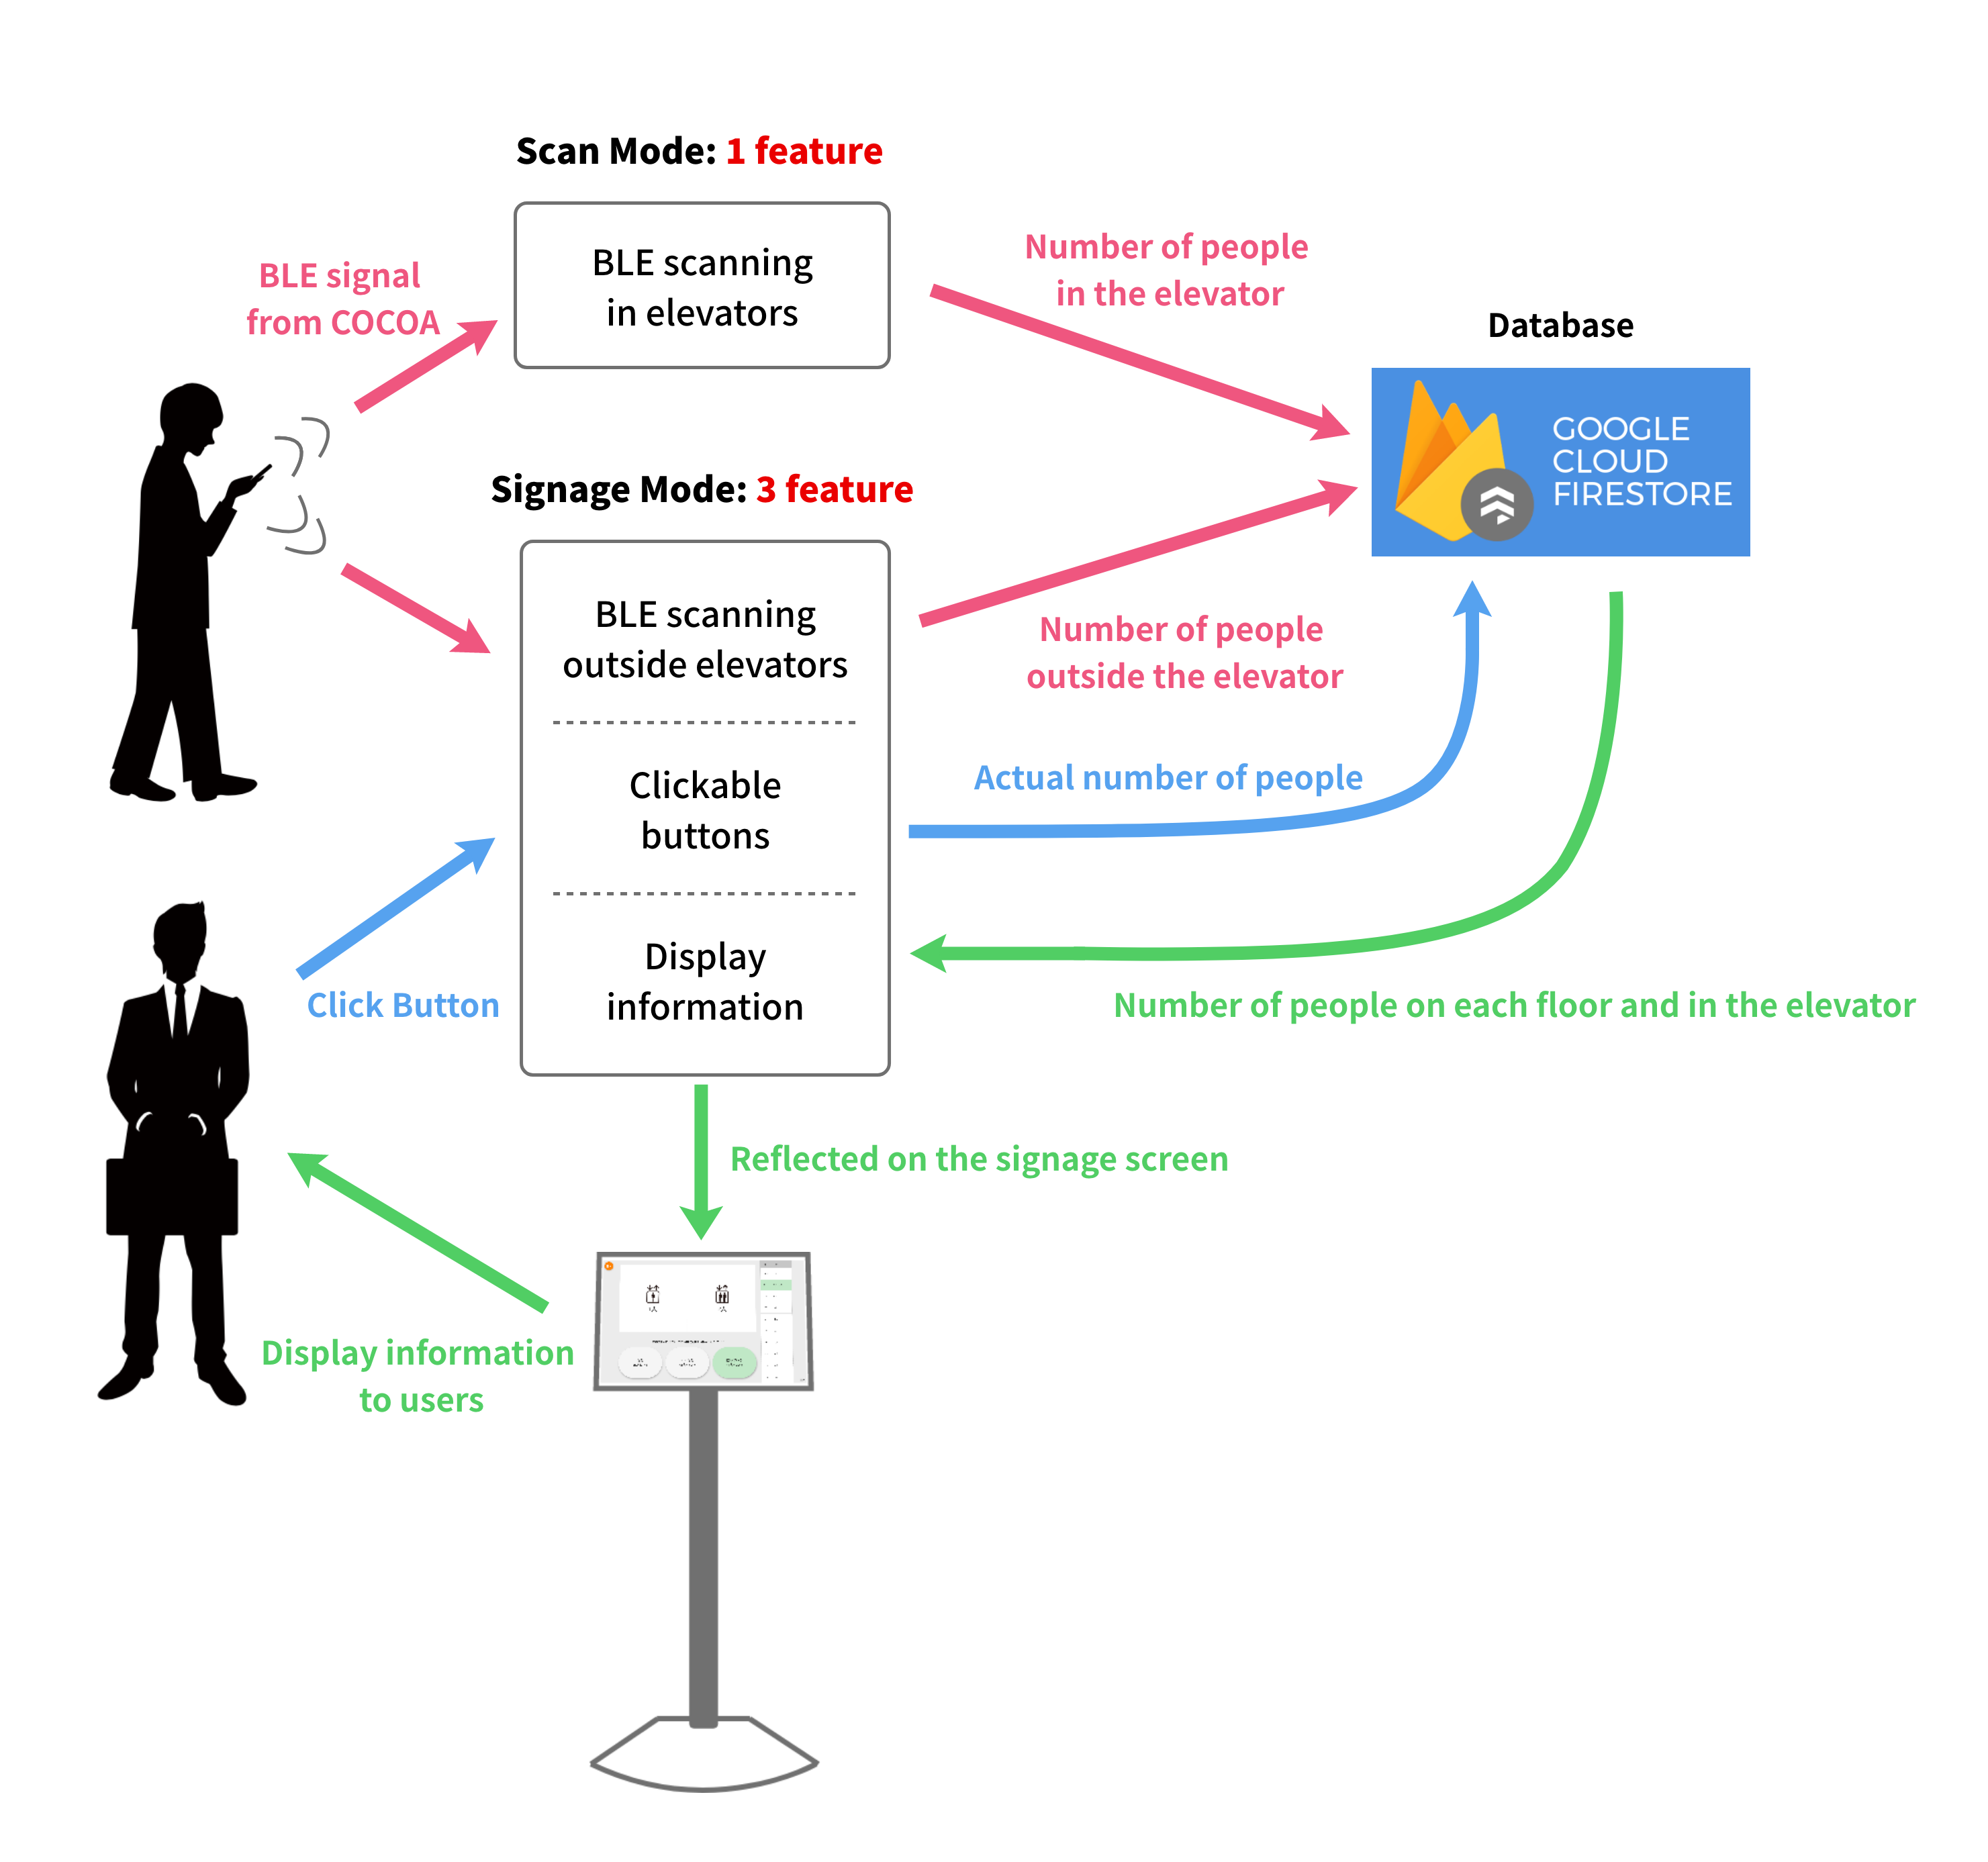
\includegraphics[clip,  width=1.0\hsize]{img/system2.png}
\caption{System configuration}
\label{fig:system2}
\end{center}
\end{figure}

% 図:アプリケーションの画面
\begin{figure}[t]
\begin{center}
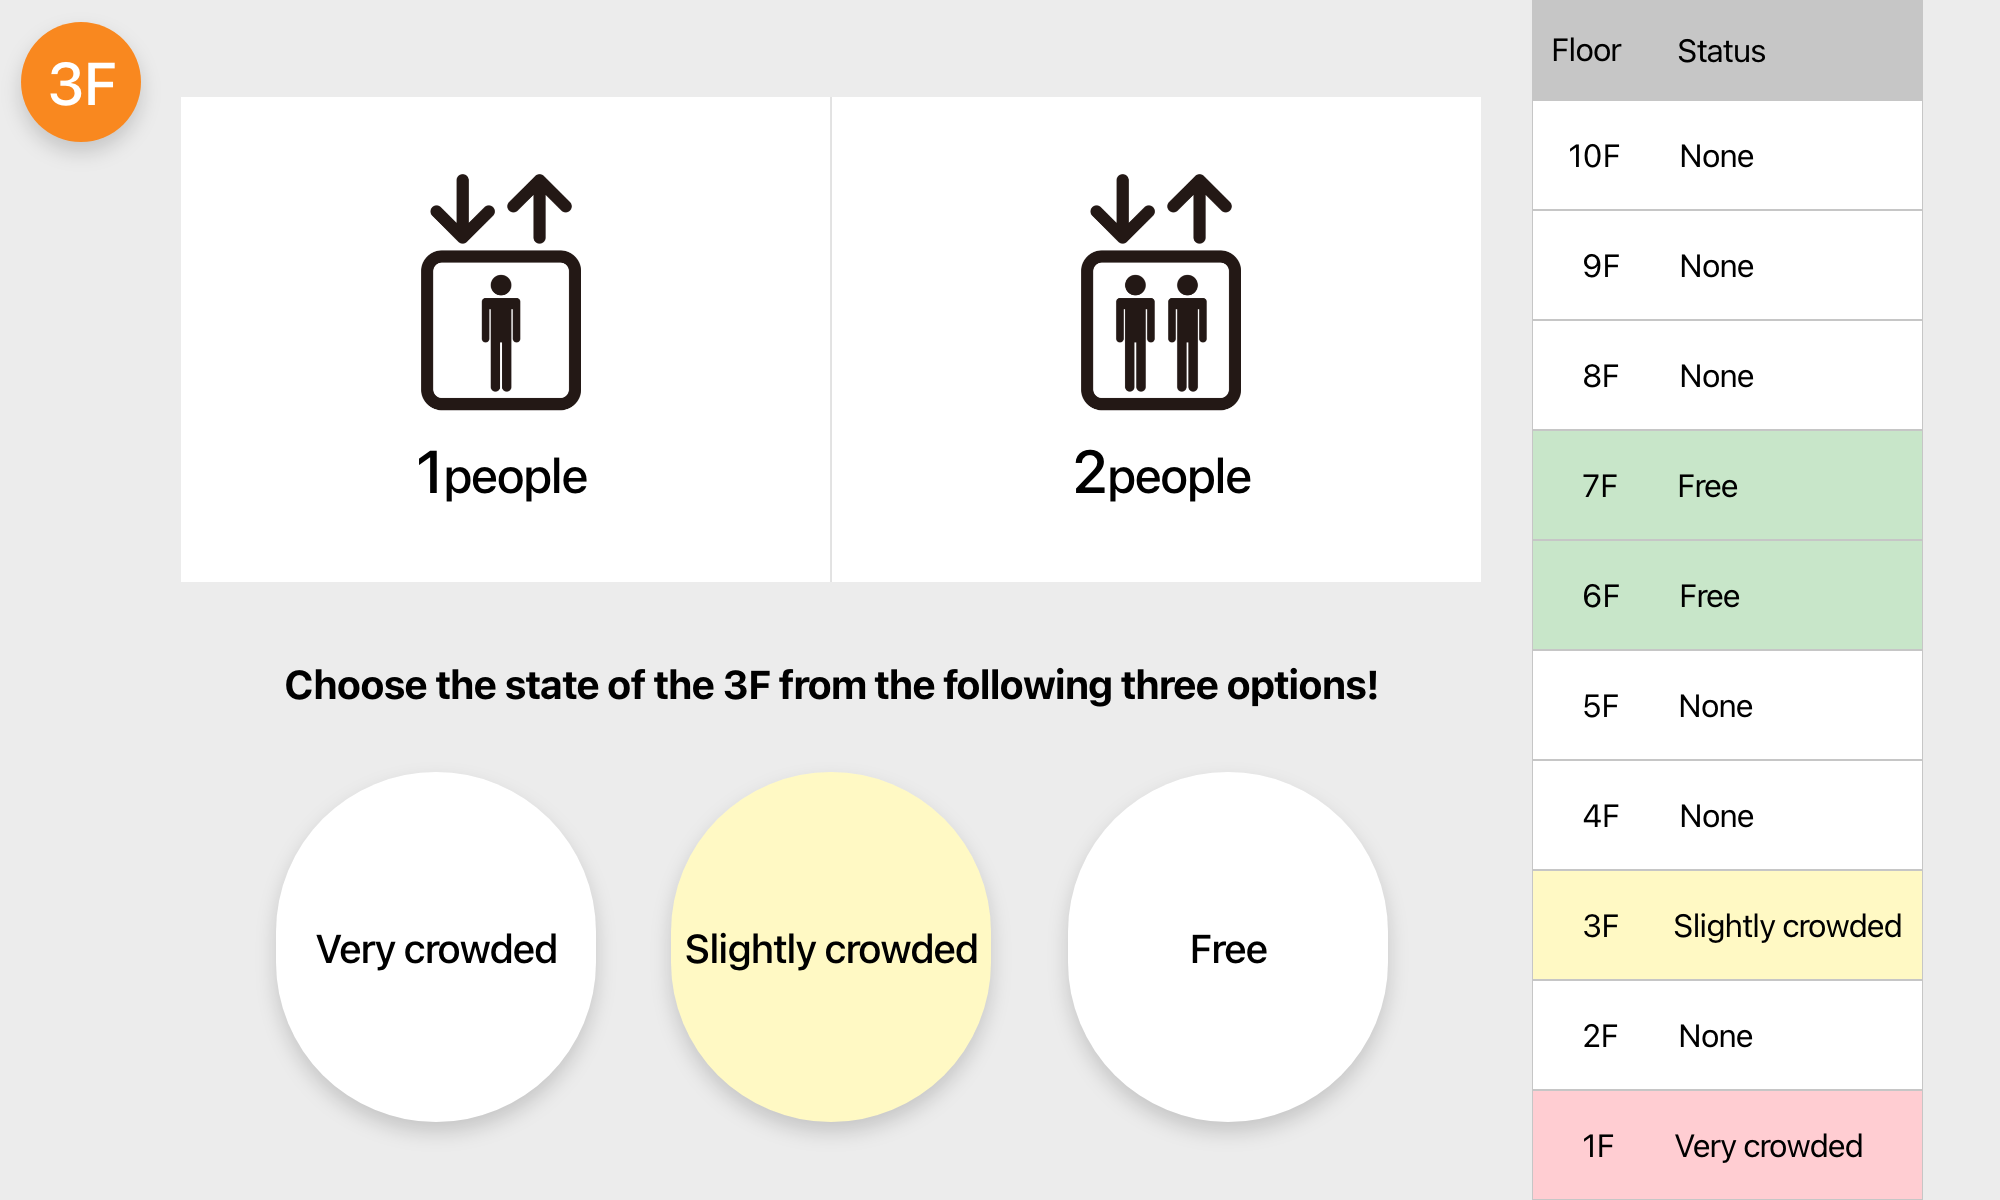
\includegraphics[clip,  width=1.0\hsize]{img/application_sceen.png}
\caption{Application screen}
\label{fig:application_sceen}
\end{center}
\end{figure}

% 図:九州大学伊都キャンパスウエスト2号館 エレベータ内
\begin{figure}[t]
\begin{center}
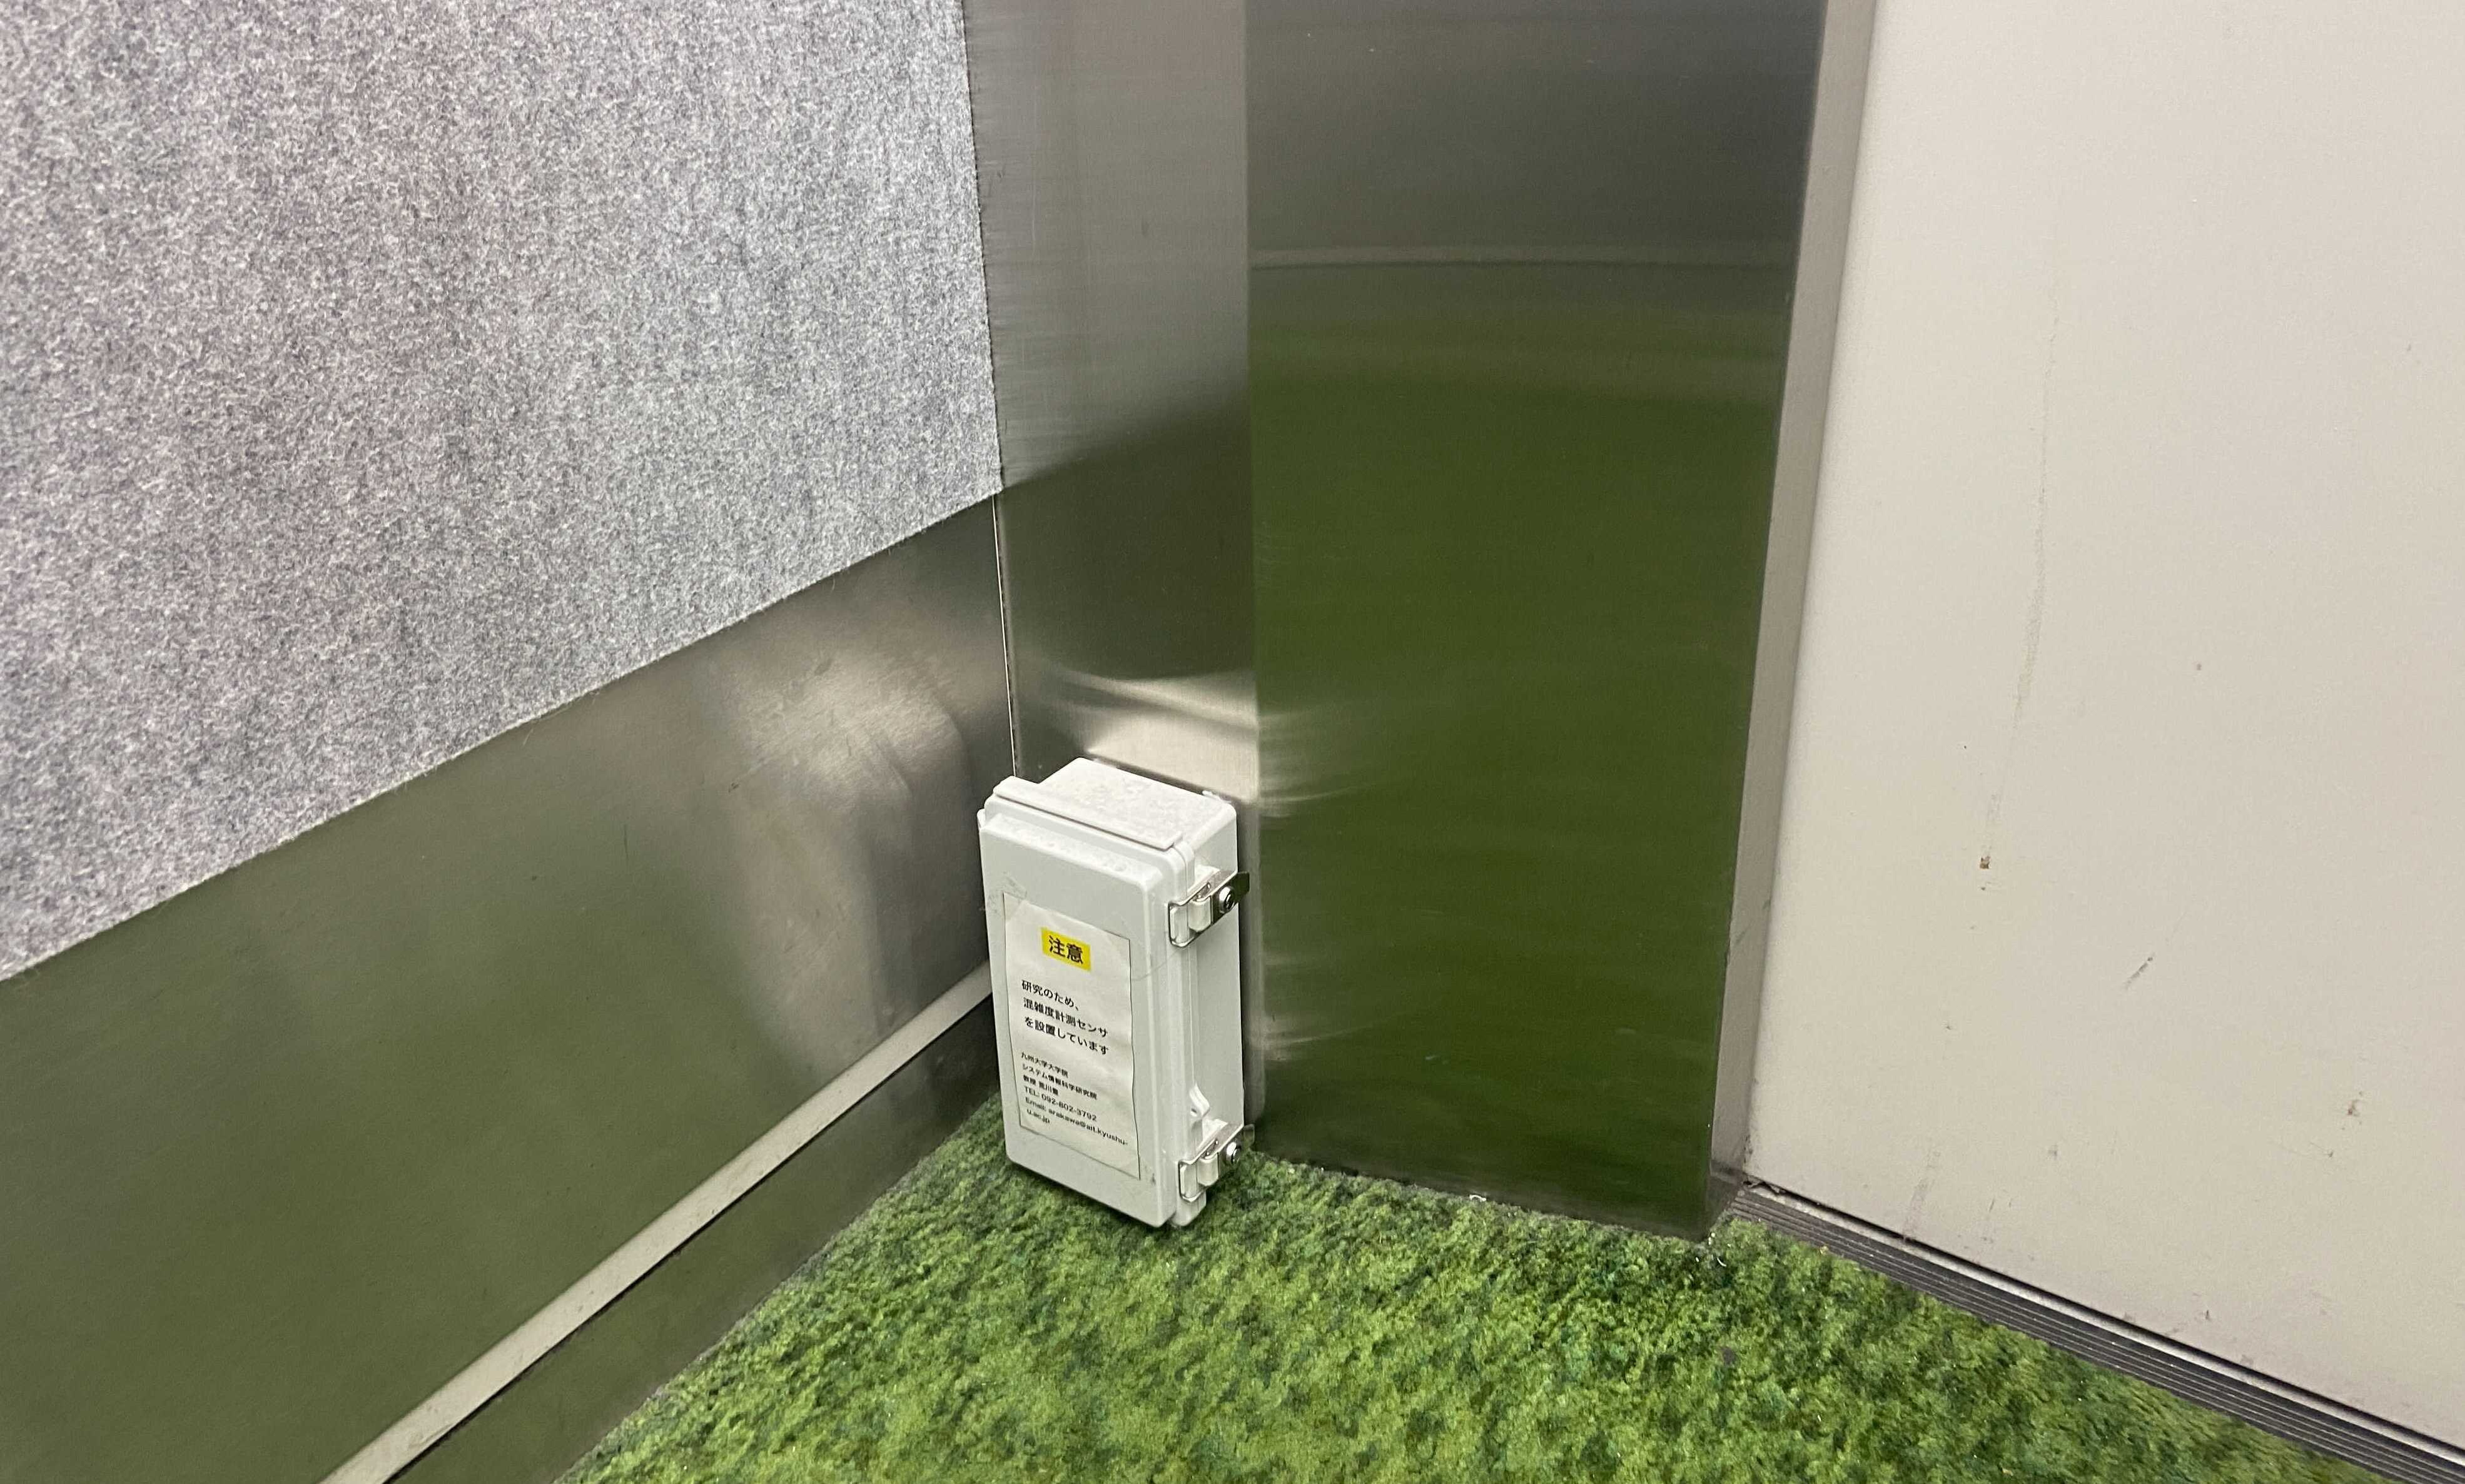
\includegraphics[clip,  width=1.0\hsize]{img/kyudai_west2_elevator_inside.jpg}
\caption{Installation of smart phones in elevators}
\label{fig:kyudai_west2_elevator_inside}
\end{center}
\end{figure}

% 図:九州大学伊都キャンパスウエスト2号館9F
\begin{figure}[t]
\begin{center}
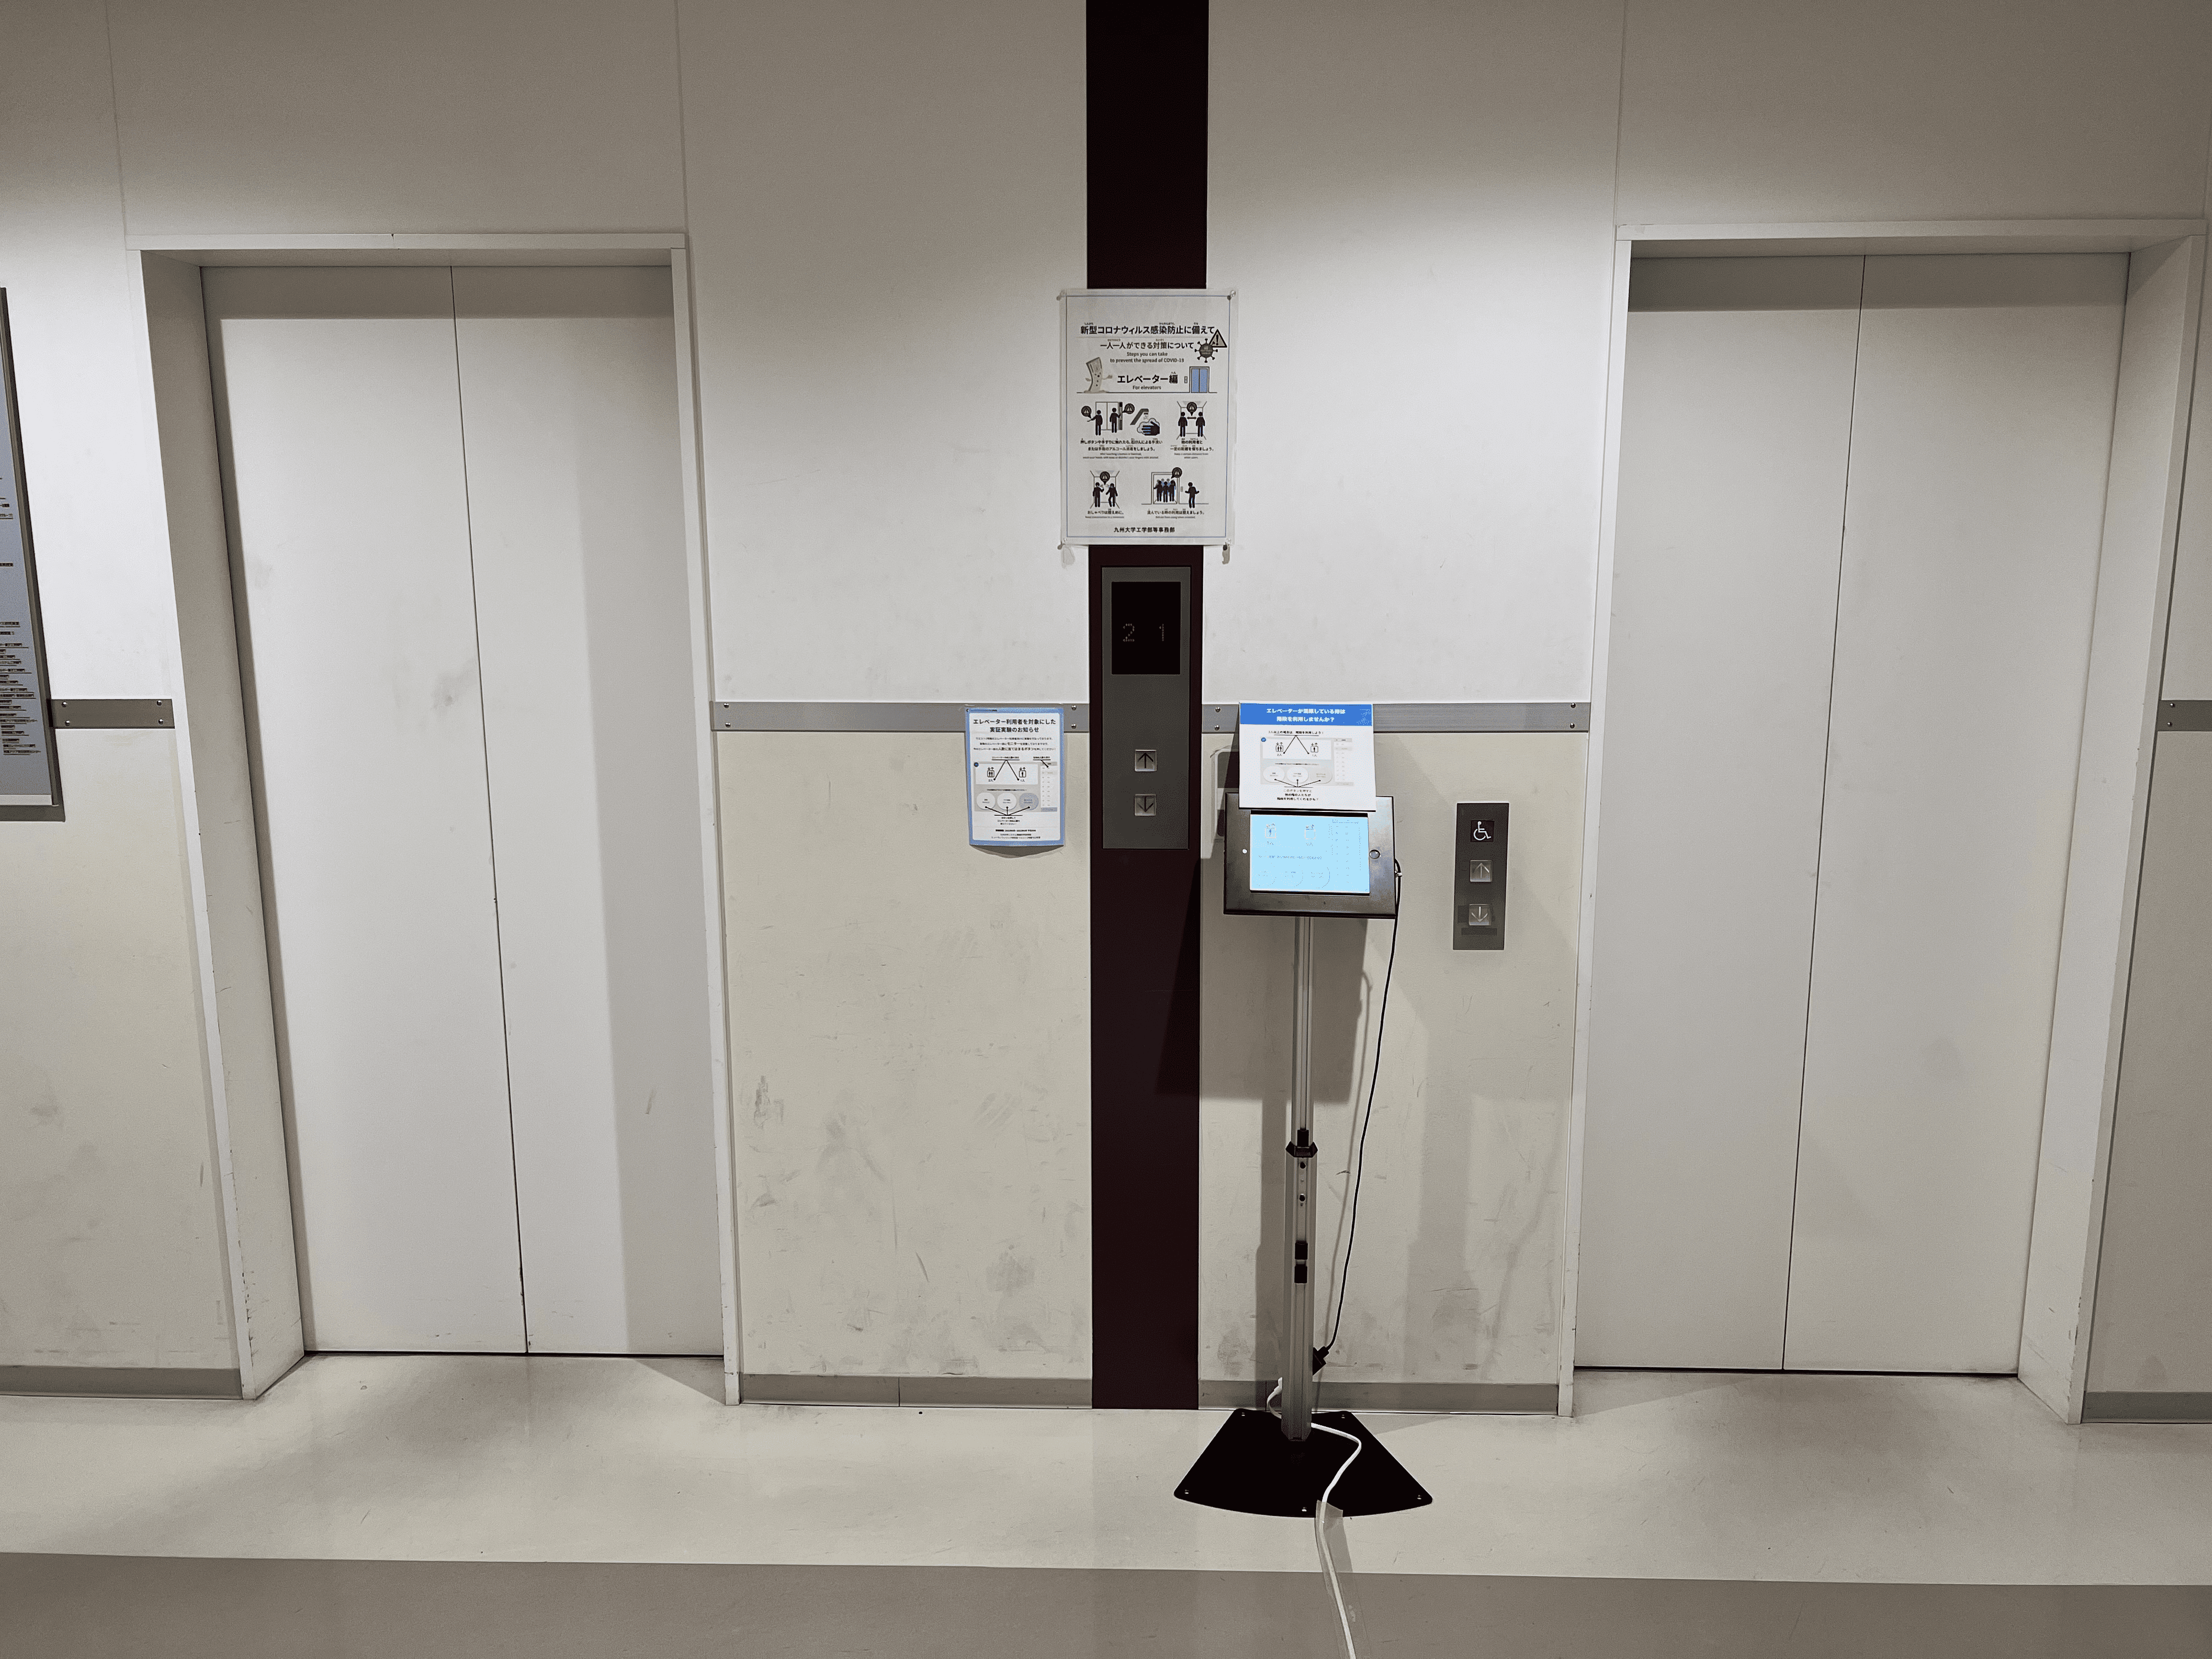
\includegraphics[clip,  width=1.0\hsize]{img/kyudai_west2_elevator.png}
\caption{Installation of tablets in the elevator hall.}
\label{fig:kyudai_west2_elevator}
\end{center}
\end{figure}

% システム実装
\subsection{System Implementation}

The configuration of this system is shown in Figure \ref{fig:system2}. The reason why we are using a smartphone as the sensor to be installed in the elevator is because we thought that an inexpensive smartphone would be suitable as a platform with built-in WiFi/BLE/LTE and a battery. The application developed in this study has a scan mode and a signage mode in one application, and can be used by simply switching between these two modes. Maintenance costs have been reduced by unifying the apps for smartphone used as sensors in elevator and tablet for displaying information. The scan mode is for smartphones installed inside the elevator (Figure \ref{fig:kyudai_west2_elevator_inside}), and only the BLE scanning function can be used. Since the basic power supply is not available in the elevator, we reduced the functions to the minimum to enable the system to operate continuously for about a day without power supply. In the signage mode, the system is designed for a tablet installed in the elevator hall (Figure \ref{fig:kyudai_west2_elevator}), and in addition to the BLE scanning function, it has a feedback function with three levels of buttons and a function to display the number of people in the elevator and the degree of congestion on each floor. In addition to the BLE scan function, this mode provides a feedback function with three levels of buttons, and a function to display the number of people in the elevator and the congestion level on each floor (Figure \ref{fig:application_sceen}). This mode basically assumes that the power can be supplied and that the lights are always on. For the implementation of the application, a framework called Flutter is used and a plugin called flutter\_blue is introduced to obtain the BLE signal.

This section describes the technical description. First of all, in order to realize Requirement 1, we detect BLE signals of -70 dBm or higher and count the number of people. However, if all BLE signals are used to count the number of people, the problem of duplicate counting of people who own multiple devices, such as Bluetooth earphones and smartphones, will occur. Therefore, we filter out only the BLE signals of COCOA to count only smartphone devices. Therefore, only the BLE signal of COCOA is filtered so that only smartphone devices are counted. The BLE standard for COCOA has been determined worldwide, and it is possible to filter only the signals of COCOA based on the values of \cite{cocoa_ble} and ServiceUUID. However, there are some problems with this method, such as the fact that the installation rate of COCOA is not 100\% and the signal strength of COCOA from Android devices is weak to begin with, making it impossible to capture enough signals. For the database, we use Cloud Firestore, and all the BLE signal data is stored in Cloud Firestore. 

Next, in order to realize Requirement 2, the number of people in the elevator and the congestion level of each floor are obtained from Cloud Firestore and displayed on the tablet screen (Figure \ref{fig:application_sceen}). In addition, in order to ask users to input the current status of the floor, the system displays the following information: crowded (more than 6 people), slightly crowded (3 people $\sim$ 5 people), and empty (1 person $\sim$ 2 people). Unlike the inside of an elevator, the elevator hall is not a shielded space, and unintended signals may be counted, so we have adopted the method of asking the users to press the buttons themselves.

%%%%%%%%%%%%%%%%%%%%%%%%%%%%%%%%%%%%%%%%%%%%%%%%%%%%%%%%%%%%%%%%%%%%%%%%
% 4. エレベータ利用者の行動パターンと待ち時間の推定
%%%%%%%%%%%%%%%%%%%%%%%%%%%%%%%%%%%%%%%%%%%%%%%%%%%%%%%%%%%%%%%%%%%%%%%%

\section{Behavior patterns of people using elevators and estimation of waiting time}
In this chapter, we describe a method to estimate the behavior pattern and waiting time of elevator users based on the time-series RSSI data of BLE signals obtained from the system described in the previous chapter.

% 図:時系列RSSIデータ
\begin{figure}[t]
  \centering
  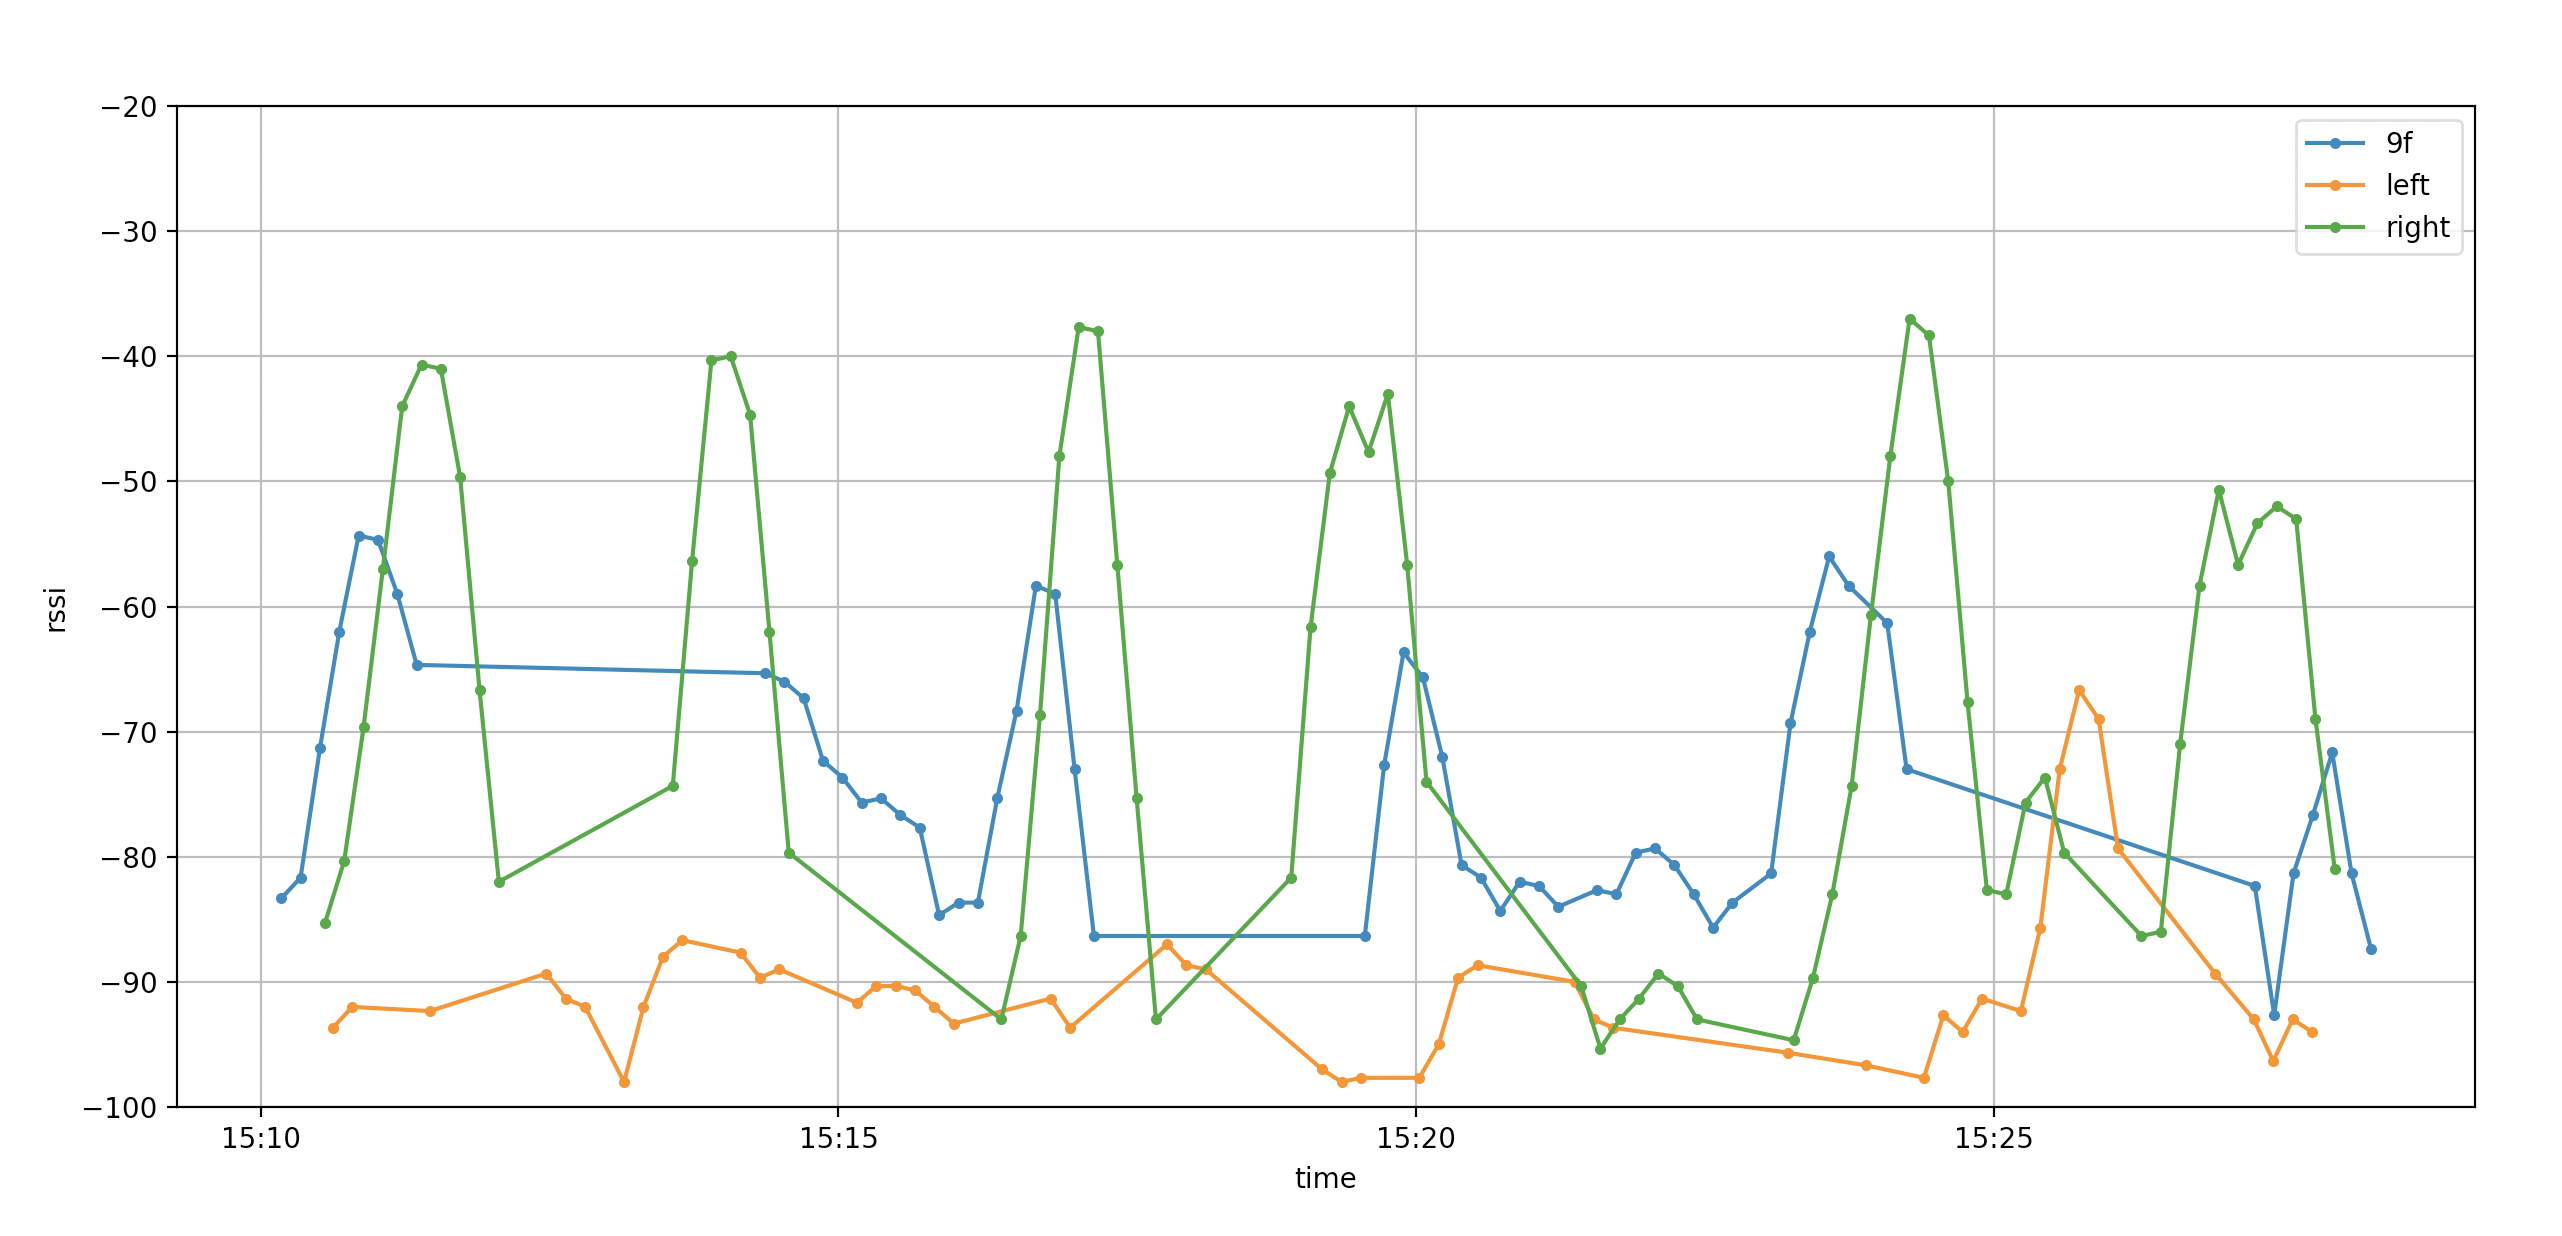
\includegraphics[width=1.0\hsize]{img/ble_rssi_original.png}
  \caption{Time series RSSI data}
  \label{fig:ble_rssi_original}
\end{figure}

% 対象とするエレベータ利用者の行動パターン
\subsection{Behavioral patterns of people who use the target elevators}

The following four types of behavioral patterns of elevator users are targeted in this study.

\begin{quote}
  \begin{itemize}
    \item Board the elevator.
    \item Exit the elevator.
    \item Use stairs instead of elevators.
    \item Passing in front of the elevator.
  \end{itemize}
\end{quote}

% 行動パターンと待ち時間を推定するアルゴリズム
\subsection{Algorithm for estimating behavior patterns and waiting times}

% MARK: don't show footnote
\thispagestyle{kisuu}

This section describes an algorithm for estimating the activity pattern described in 4.1 from time-series RSSI data.
Let $A_{hall}$, $A_{right}$, and $A_{left}$ be the time-series RSSI data acquired from the tablet installed in front of the elevator hall, the smartphone installed in the elevator on the right, and the smartphone installed in the elevator on the left, respectively. In $A_{hall}$, $T_{start}$ is the time when the RSSI value reaches -70 dBm or higher. Let $T_{end}$ be the time when the RSSI value drops more than 10 dBm from the maximum value. Let the time 10 seconds before $T_{start}$ be $T_{start}'$ and the time 10 seconds after $T_{end}$ be $T_{end}'$, and let the data of $A_{right}$ and $A_{left}$ from $T_{start}'$ to $T_{end}'$ be $A_{right}'$ and $A_{left}'$. If the maximum RSSI values of $A_{right}'$ and $A_{left}'$ are both below -70 dBm, it is judged that ''Use stairs instead of elevators'' or ''Passing in front of the elevator''. If the maximum value of RSSI of $A_{right}'$ is higher than that of $A_{left}'$, it is judged as ''boarded the elevator on the right side'' or ''got off from the elevator on the right side'', and if it is lower than that, it is judged as ''boarded the elevator on the left side'' or ''got off from the elevator on the left side''. If the time at which the RSSI value of $A_{right}'$ reaches the maximum is later than the time at which the RSSI value of $A_{hall}$ reaches the maximum, it is judged to be ''boarding the right elevator'', and if it is earlier, it is judged to be ''getting off from the right elevator''. The same procedure is applied to ''getting on the left elevator'' or ''getting off from the left elevator''. In the case of ''getting on the elevator'', the difference between $T_{start}$ and $T_{end}$ is regarded as the waiting time.


% 実験方法
\subsection{Experimental Methods}

The experiment is conducted in the elevator on the 9th floor of the West 2 Building of Kyushu University, Ito Campus (Figure \ref{fig:kyudai_west2_elevator}). In this experiment, two kinds of behavioral patterns, ''getting on the elevator on the right side'' and ''getting off the elevator on the right side'', were reproduced and tested with an iPhone with COCOA installed. The experimental method is described below.

% MARK: don't show footnote
\thispagestyle{guusuu}

First, the participants pushed the ''get off'' button in front of the elevator hall on the 9th floor and waited in front of the elevator on the right side until the elevator arrived. Get on the elevator, move to the first floor, and get off the elevator. After waiting for a minute or two, press the ascending button in front of the elevator hall on the first floor and follow the same procedure to the ninth floor. Repeat this procedure for three sets. Record the time you press the elevator button, the time you get on the elevator, and the time you get off the elevator (\tablename\ref{table:record_table}).


% 実験結果
\subsection{Experimental results}

The time series RSSI data from 15:10:00 to 15:30:00 obtained from the tablet terminals in front of the elevator hall on the 9th floor and the smartphone terminals installed in the elevators on the right and left sides are shown in Figure \ref{fig:ble_rssi_original}.
Based on the algorithm, the detection rate of boarding and alighting was 100\%. The estimated waiting time on the 9th floor when a passenger gets on the train is shown in Figure \ref{fig:ble_rssi_9f_wait}, Figure \ref{fig:ble_rssi_9f_wait_quess} and \tablename\ref{table:record_table_guess}. Compared to \tablename\ref{table:record_table}, the estimated wait times are roughly consistent, although there may be a time lag of 5 to 10 seconds between the estimated start time ($T_{start}$) and estimated end time ($T_{end}$). Currently, the timing of the BLE scan is assumed to be about once every 10 seconds, but if the interval of the scan is shortened, the accuracy is expected to be improved.

% MARK: don't show footnote
\thispagestyle{kisuu}

% 表:実験の記録
\begin{table*}[ht]
  \caption{Record of the experiment}
  \label{table:record_table}
  \begin{tabular}{c|ccc|c}
    \hline
    \textbf{\begin{tabular}{c}behavioral \\ pattern\end{tabular}} &
    \textbf{\begin{tabular}{c}Time when \\ the elevator button \\ is pressed\end{tabular}} &
    \textbf{\begin{tabular}{c}Time of \\ the elevator \\ ride\end{tabular}} &
    \textbf{\begin{tabular}{c}Time \\ you got off \\ the elevator\end{tabular}} &
    \textbf{\begin{tabular}{c}waiting \\ time\end{tabular}}                                          \\
    \hline\hline
    Move from 9F to 1F                 & 15:10:31 & 15:11:01 & 15:11:22 & 30sec \\
    Move from 1F to 9F                 & 15:13:20 & 15:13:45 & 15:14:10 & 25sec \\
    Move from 9F to 1F                 & 15:16:32 & 15:16:50 & 15:17:22 & 18sec \\
    Move from 1F to 9F                 & 15:19:00 & 15:19:12 & 15:19:43 & 12sec \\
    Move from 9F to 1F                 & 15:23:17 & 15:23:58 & 15:24:34 & 41sec \\
    Move from 1F to 9F                 & 15:25:55 & 15:26:42 & 15:27:32 & 47sec \\
    \hline
  \end{tabular}
\end{table*}

% 図:時系列RSSIデータと9Fでの待ち時間
\begin{figure}[t]
  \centering
  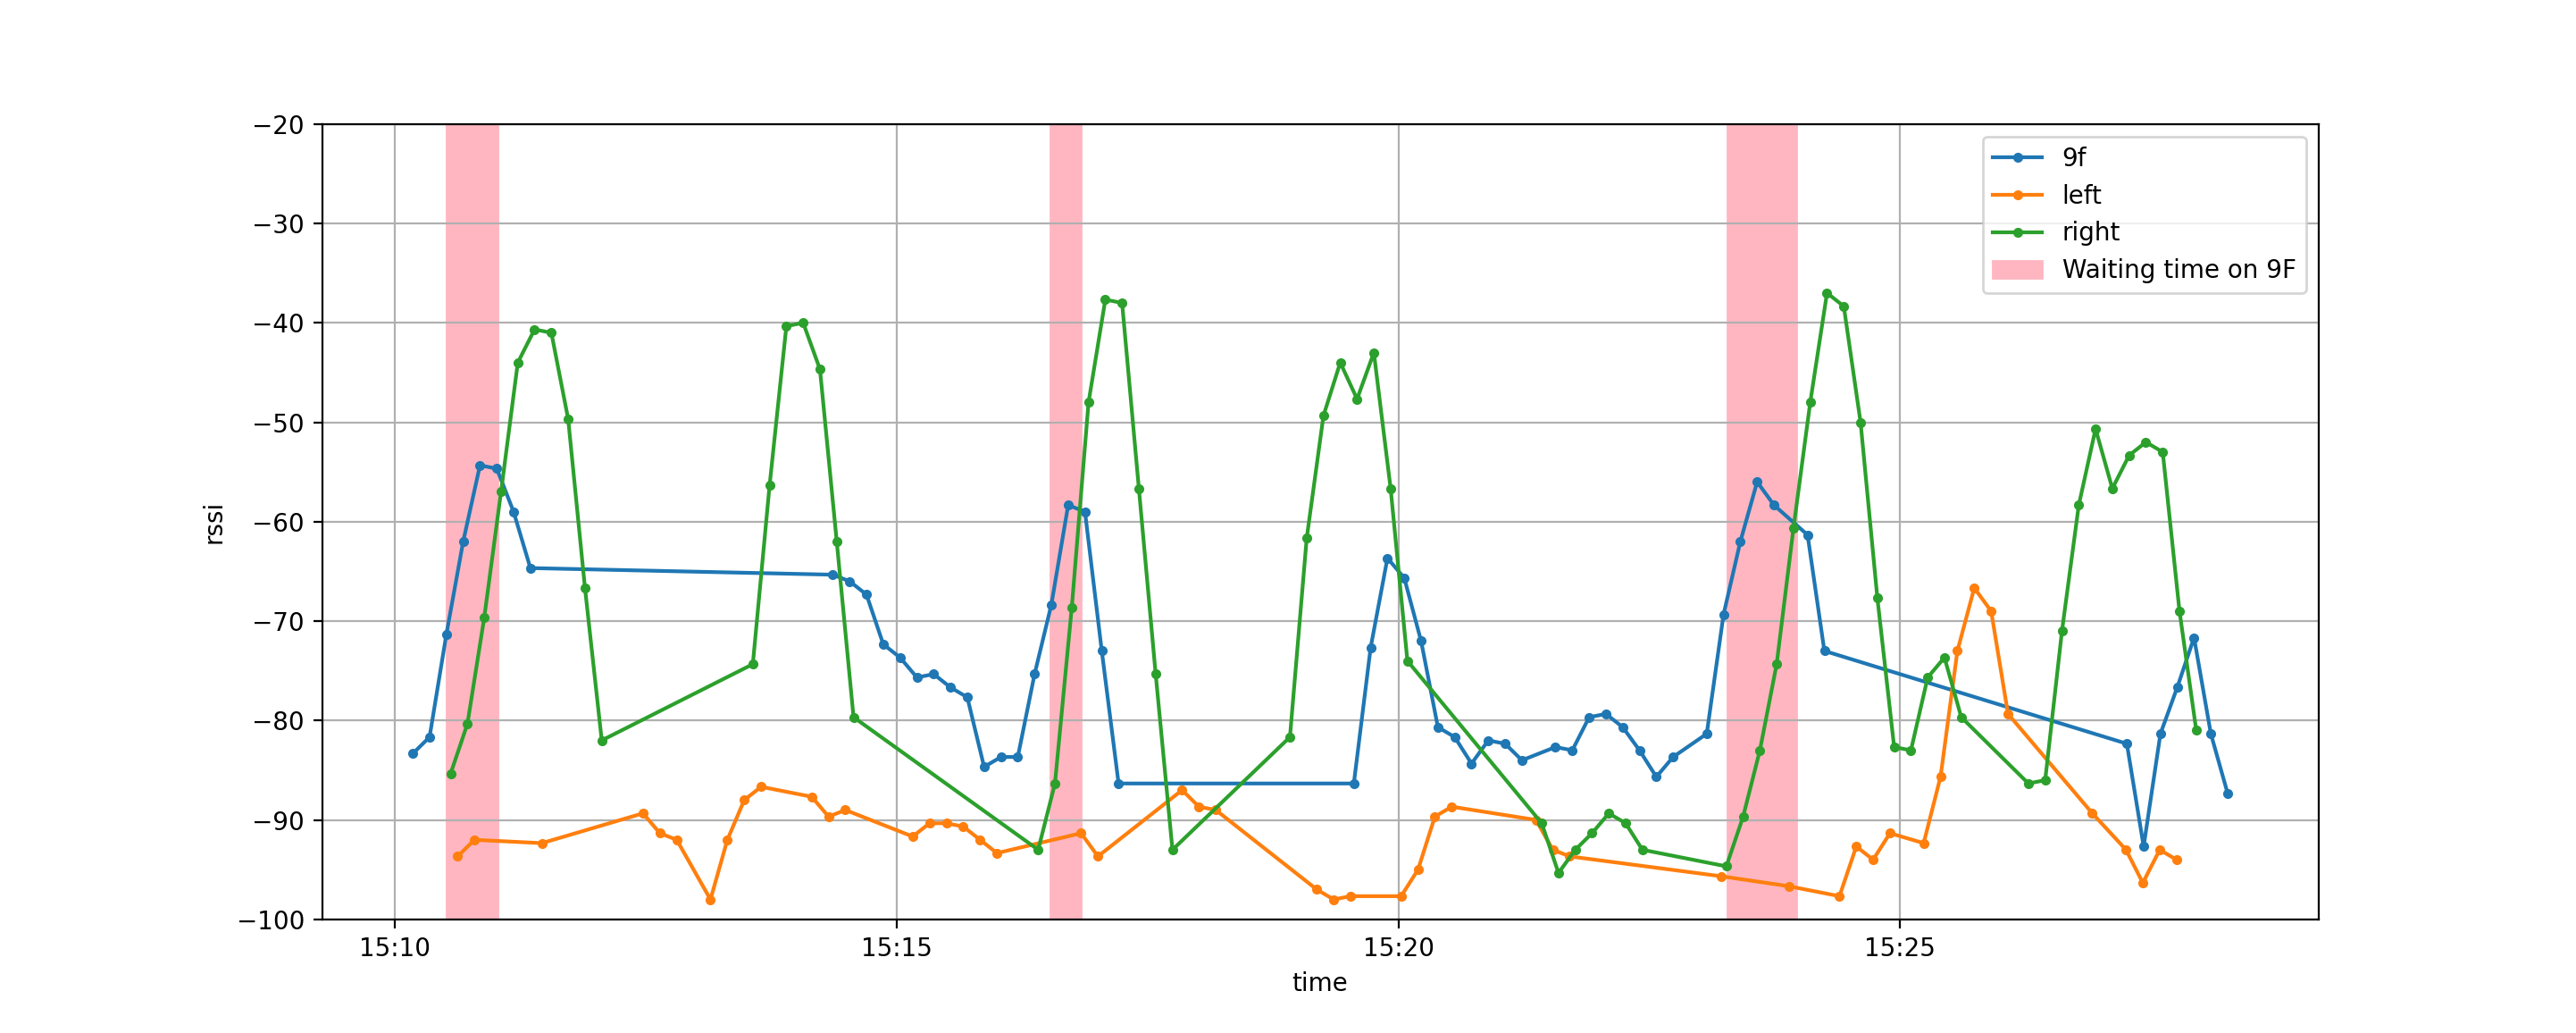
\includegraphics[width=1.0\hsize]{img/ble_rssi_9f_wait.png}
  \caption{Time series RSSI data and waiting time at 9F and Actual waiting time}
  \label{fig:ble_rssi_9f_wait}
\end{figure}

% 図:時系列RSSIデータと9Fでの待ち時間(推定値)
\begin{figure}[t]
  \centering
  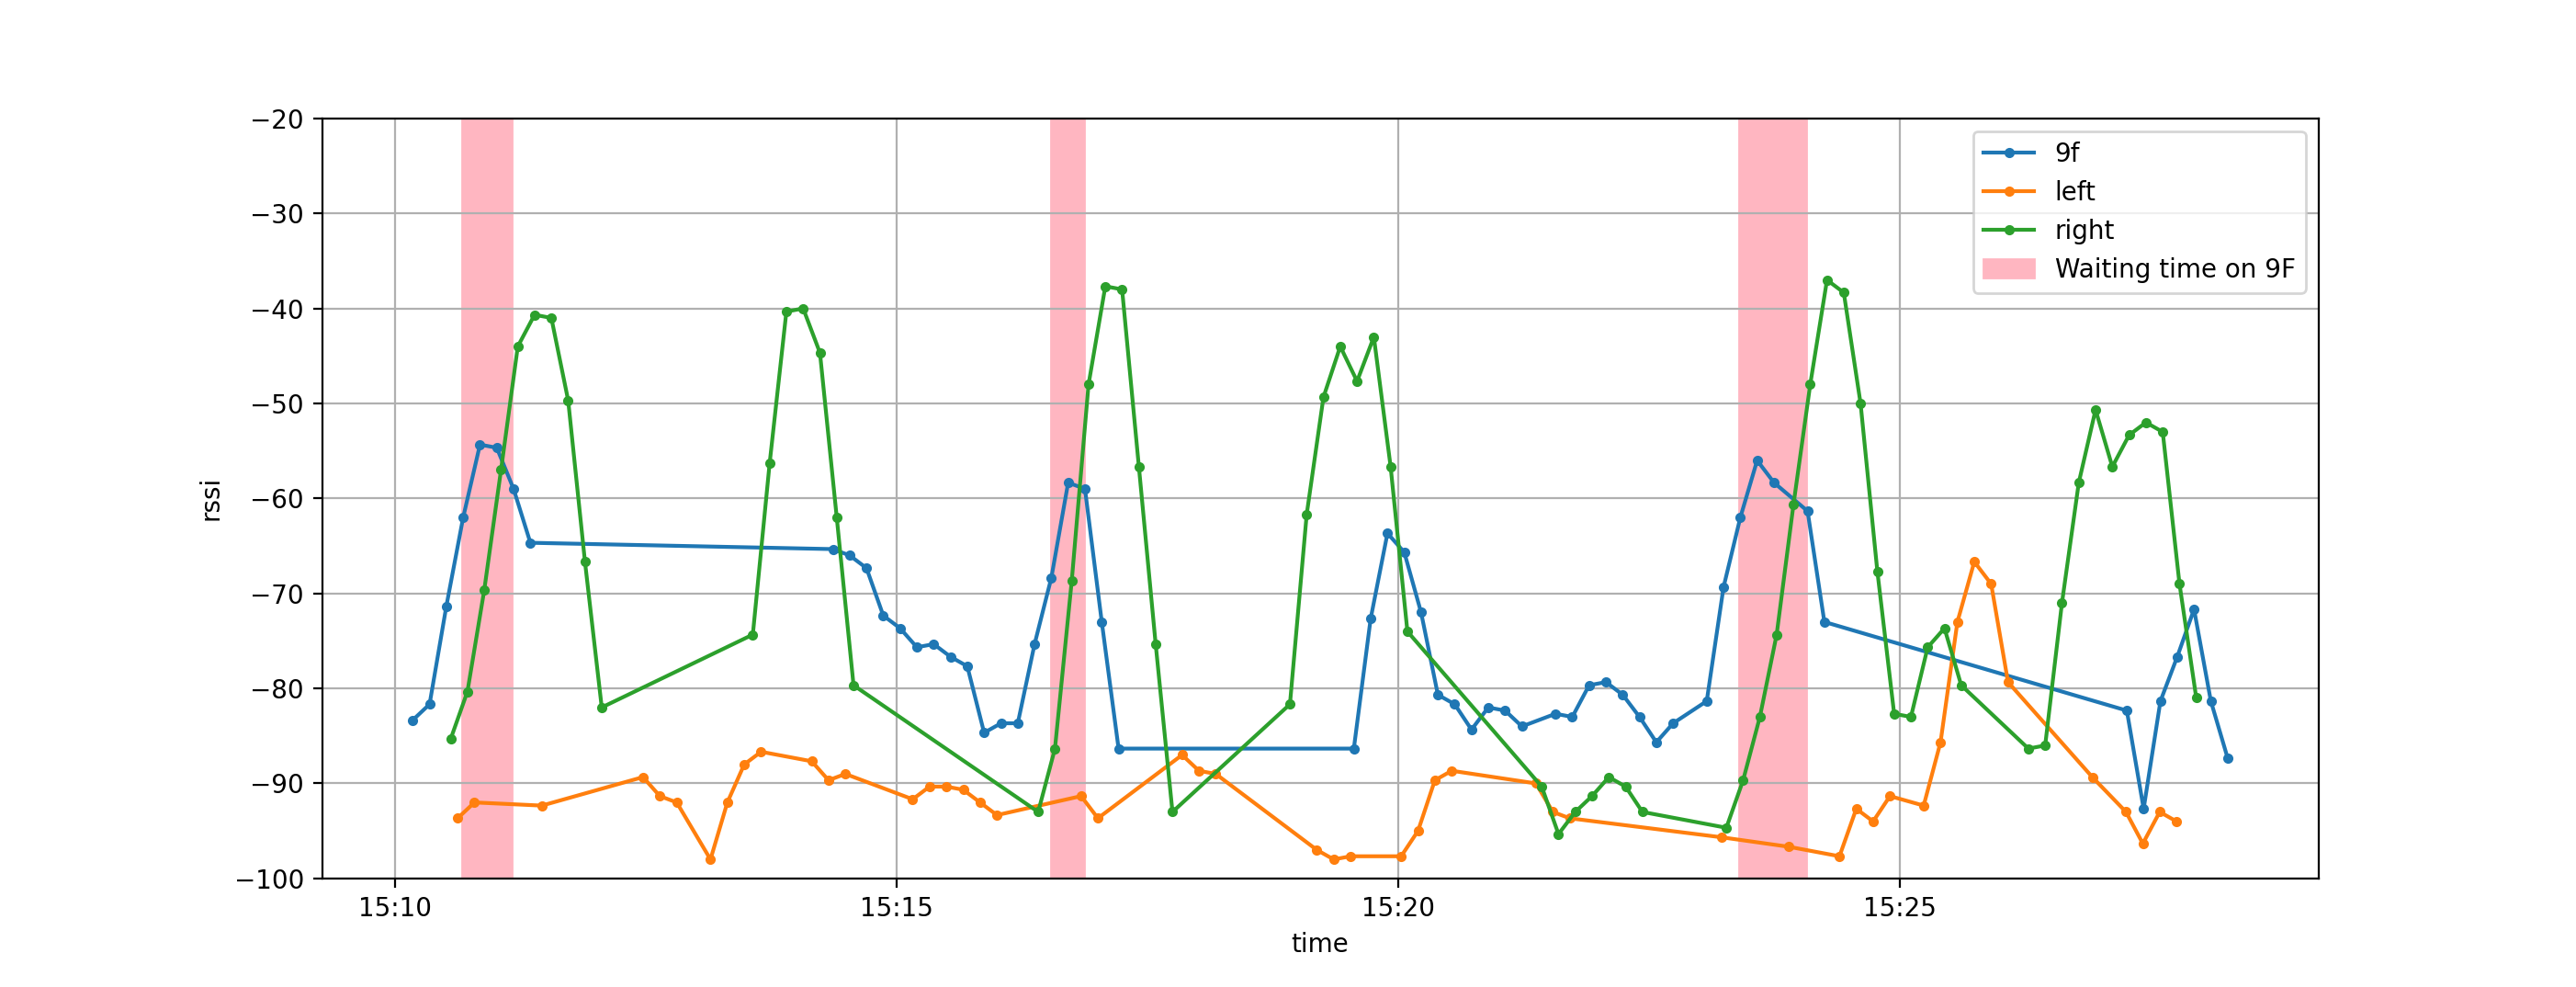
\includegraphics[width=1.0\hsize]{img/ble_rssi_9f_wait_guess.png}
  \caption{Time series RSSI data and waiting time at 9F and Estimated latency by algorithm}
  \label{fig:ble_rssi_9f_wait_quess}
\end{figure}

% 表:アルゴリズムによる推定待ち時間
\begin{table*}[ht]
  \caption{Estimated latency by algorithm}
  \label{table:record_table_guess}
  \centering
  \begin{tabular}{c|cc|c}
    \hline
    \textbf{behavioral pattern} & \textbf{$T_{start}$} & \textbf{$T_{end}$} & \textbf{Estimated waiting time} \\ \hline\hline
    Take the right elevator.    & 15:10:40             & 15:11:10           & 30sec                           \\
    Take the right elevator.    & 15:16:32             & 15:16:52           & 20sec                           \\
    Take the right elevator.    & 15:23:24             & 15:24:04           & 40sec                           \\
    \hline
  \end{tabular}
\end{table*}

%%%%%%%%%%%%%%%%%%%%%%%%%%%%%%%%%%%%%%%%%%%%%%%%%%%%%%%%%%%%%%%%%%%%%%%%
% 5. おわりに
%%%%%%%%%%%%%%%%%%%%%%%%%%%%%%%%%%%%%%%%%%%%%%%%%%%%%%%%%%%%%%%%%%%%%%%%
\section{Conclusion}
In this paper, we developed a system that measures the number of people in an elevator by measuring the COCOA signal, and visualizes in real time the congestion in the elevator and on each floor. We hypothesize that visualization of congestion to elevator users will encourage them to make a decision not to use the elevator. In the future, we plan to examine the long-term effect of this system on the increase or decrease of elevator utilization rate during congestion with and without this system. Furthermore we plan to integrate feedback mechanisms into our system to encourage behavioral changes, such as using the stairs instead of the elevator based on the IoT data-driven nudging concept \cite{nakamura2021iot}.


\subsubsection{Acknowledgements.}
This work was supported in part by JSPS Grant-in-Aid for Scientific Research JP18H03233 and NEDO Research and Development of My-IoT Development Platform (JPNP18014).

% MARK: don't show footnote
\thispagestyle{guusuu}

%
% ---- Bibliography ----
%
% BibTeX users should specify bibliography style 'splncs04'.
% References will then be sorted and formatted in the correct style.
%

% ----------------------------------------------------------------
% MARK: エラー発生により, bibファイルは使用できない
% Recipe returns with error: 12/null. PID: 43899. message: Latexmk: Run number 1 of rule 'pdflatex'
% Latexmk: Non-existent bbl file '/Users/alesion30/work/latex/bcss2022-elevator/out/main.bbl in line'
% ----------------------------------------------------------------
% \bibliographystyle{splncs04}
% \bibliography{myreference}
\begin{thebibliography}{8}
  \bibitem{research_camera}
  Arai, H., Ito, N., Taniguti, N.: Image processing techniques for capturing
  crowds at a macroscopic level - estimating the number of people based on
  geometric models of people and crowds and its applications. Tech. Rep.~13,
  NTT Media Intelligence Laboratory, NTT Media Intelligence Laboratory, NTT
  Media Intelligence Laboratory (jan 2014)

  \bibitem{kajima}
  Corporation, K.: Smart buildings support workers' health behaviors.
  "\url{https://www.kajima.co.jp/news/press/202107/6a1-j.htm}"

  \bibitem{elenavi}
  Corporation, M.E.: Solving elevator congestion with ele-navi.
  "\url{https://www.mitsubishielectric.co.jp/elevator/nayami/002/}"

  \bibitem{cocoa_ble}
  Google: Contact tracing - bluetooth specification v1.1.
  "\url{https://blog.google/documents/58/Contact\_Tracing\_-\_Bluetooth\_Specification\_v1.1\_RYGZbKW.pdf}"

  \bibitem{ministry}
  Japan, P.M.O.O.: Prime minister's residence.
  "\url{https://www.kantei.go.jp/jp/content/000062771.pdf}"

  \bibitem{kanamitu-2021-dicomo}
  Kanemitu, Y., TAYA, E., Tachibana, K., Nakamura, Y., Matuda, Y., Suwa, H.,
  Yasumoto, K.: Estimating congestion on a bus route using ble. In: Information
  Processing Society of Japan DICOMO Symposium (2021)

  \bibitem{komai2016beacon}
  Komai, K., Fujimoto, M., Arakawa, Y., Suwa, H., Kashimoto, Y., Yasumoto, K.:
  Beacon-based multi-person activity monitoring system for day care center. In:
  2016 IEEE International Conference on Pervasive Computing and Communication
  Workshops (PerCom Workshops). pp.~1--6. IEEE (2016)

  \bibitem{komai2016elderly}
  Komai, K., Fujimoto, M., Arakawa, Y., Suwa, H., Kashimoto, Y., Yasumoto, K.:
  Elderly person monitoring in day care center using bluetooth low energy. In:
  2016 10th International Symposium on Medical Information and Communication
  Technology (ISMICT). pp.~1--5. IEEE (2016)

  \bibitem{ipsj-taikai-2020-matsumoto}
  Matumoto, T., Takahashi, R., Ishida, S., Arakawa, Y.: Initial evaluation of
  device-free indoor congestion estimation using wireless lan. In: The 82nd
  National Convention of Information Processing Society of Japan (2020)

  \bibitem{nakamura2021iot}
  Nakamura, Y., Matsuda, Y.: Iot nudge: Iot data-driven nudging for health
  behavior change. In: Adjunct Proceedings of the 2021 ACM International Joint
  Conference on Pervasive and Ubiquitous Computing and Proceedings of the 2021
  ACM International Symposium on Wearable Computers. pp. 51--53 (2021)

  \bibitem{misc/26987957}
  Suzuki, Y., Manato, M., Yoshino, K., Hidaka, M., Mai, N.Q., Nagano, K.,
  Nakamura, Y., Otubo, A., Tanaka, S., Yasumoto, K., Nakamura, T.: Construction
  of iot2h tourism information application for kyoto inbound tourism. The 11th
  Forum on Data Engineering and Information Management (DEIM2019)  (3 2019)

  \bibitem{research_elevator_log}
  Taguchi, H., Suzuki, N., Shikai, M.: Estimating passenger queue length based on
  elevator control log. In: IEICE Conferences Archives. The Institute of
  Electronics, Information and Communication Engineers (2015)

  \bibitem{research_itocon}
  Takahashi, R., Hayashi, K., Mitsukude, Y., Ninomata, M., Inoue, S., Matsuo, S.,
  Ishida, S., Arakawa, Y., Takano, S.: Bus stop congestion visualization system
  itocon. In: Proceedings of the 28th Workshop on Multimedia Communication and
  Distributed Processing. pp. 227--230 (nov 2020)

  \bibitem{research_elevator_camera}
  Uchidate, H., Inoda, R., Tsuji, T., Abe, S.: Counting people and recognition of
  wheelchairs at elevator lobby by real-time image processing. IEEJ
  Transactions D (Journal of Industrial Application Division)  \textbf{129}(6),
  578--584 (2009)

  \bibitem{umeki2018real}
  Umeki, K., Nakamura, Y., Fujimoto, M., Arakawa, Y., Yasumoto, K.: Real-time
  congestion estimation in sightseeing spots with ble devices. In: 2018 IEEE
  International Conference on Pervasive Computing and Communications Workshops
  (PerCom Workshops). pp. 430--432. IEEE (2018)
\end{thebibliography}


% MARK: don't show footnote
\thispagestyle{guusuu}

\end{document}
